\chapter{Marco teórico y objetivos del trabajo}
\iffalse
\begin{chapquote}{Autor, \textit{tiempo}}
`` cita''
\end{chapquote}
\fi

\iffalse
\section{La visión como herramienta}
\subsection{La visión en el ser humano}
El ser humano es capaz de interactuar con el mundo que le rodea de diversas maneras mediante los sentidos: tacto, gusto, oído, olfato y por último pero no menos importante la visión. Este último sentido nos permite recoger gran cantidad de información de nuestro entorno, procesarla y actuar en consecuencia. 

Lejos de realizar un estudio anatómico del sentido de la vista en el ser humano, se disponen a continuación ciertas características de interés que permiten apreciar su potencia.
\\
Una de las primeras cuestiones que se vienen a la mente cuando se habla de la ``simple vista'' es su resolución, es decir, cuál es la mínima distancia que es capaz de distinguir. Se puede estudiar mediante la resolución angular que para el ser humano se encuentra entorno a 1' o 2' o lo que es lo mismo un intervalo de 0,02º a 0,03º\cite{simple_vista}. Dicho de otra forma, un ojo humano sano y correctamente desarrollado puede distinguir objetos de entre 30cm y 60cm a 1km de distancia. Por ejemplo, una persona podría detectar dos balones de playa de un diámetro aproximado de 45cm hasta 1km de distancia.

%https://es.wikipedia.org/wiki/Simple_vista

El campo de visión es también un aspecto importante ya que determina la cantidad de información que los ojos pueden recibir en un instante dado. El ``cono de visión'' queda entorno a unos 130º en vertical y 160º en horizontal que equivale aproximadamente a una lente con longitud focal de 2mm\cite{angle_of_view}. Se entiende como distancia focal, en el ámbito de la fotografía, la distancia entre el punto en el que convergen los rayos de luz formando una imagen y el sensor digital del dispositivo obteniendo esta medida cuando la lente está enfocada al infinito.

En resumidas cuentas, a mayor distancia focal, más estrecho será el ángulo de visión y mayor la magnificación ocurriendo el efecto contrario según se reduce la distancia focal. Se muestra en la figura \ref{fig:focal_length} un esquema de lo explicado. 


\begin{figure}[!htb]
\centering
\minipage{0.7\textwidth}
  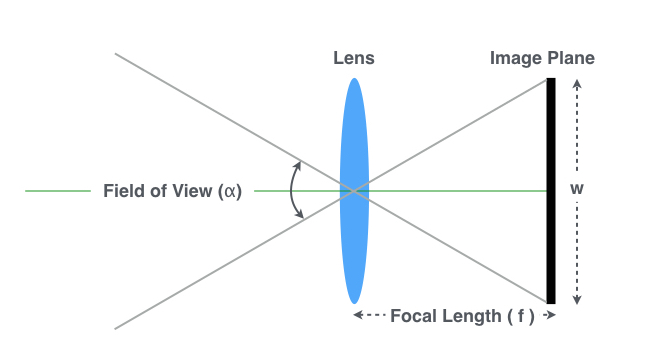
\includegraphics[width=\linewidth]{focal_length}
  \caption{Ángulo de visión $\alpha$ en función de la distancia focal $f$}\label{fig:focal_length}
\endminipage\hfill

\end{figure}

%https://en.wikipedia.org/wiki/Angle_of_view#Common_lens_angles_of_view


Por último, se considera la velocidad de enfoque o acomodación del ojo humano. Según un experimento llevado cabo por el Massachussets Institute of Technology (MIT)\cite{mit_experiment} el ojo humano es capaz de captar una imagen para su posterior procesamiento en tan solamente 13 milisegundos.


%http://www.sophimania.pe/ciencia/cerebro-y-neurociencias/estudio-revela-que-el-ojo-humano-capta-una-imagen-en-13-milisegundos/
%http://news.mit.edu/2014/in-the-blink-of-an-eye-0116

Se ha planteado entonces una situación en la que hay un instrumento de gran precisión y prolongada durabilidad embarcado en un ser vivo falible y errático. No sólo esto sino que nunca se llega a dominar por completo el manejo de éste órgano así como su uso en conjunto a las demás partes del cuerpo y siempre todo ello limitado por la velocidad de respuesta que puede proporcionar el sistema nervioso.

\subsection{Exportando la capacidad de visión}

Una vez descritas brevemente la potencia, capacidad y posibilidades que aporta la visión en el ser humano, se puede ir más allá, subir un nivel y dotar a entes ajenos al hombre de la habilidad de obtener y procesar información visual. Este concepto existe desde finales de la década de los sesenta y puede introducirse como visión artificial o visión por computador\cite{vision_artificial}:
\\
``Disciplina científica que incluye métodos para adquirir, procesar, analizar y comprender las imágenes del mundo real con el fin de producir información numérica o simbólica para que puedan ser tratados por un computado''
\\
Esta forma de trabajar con información visual es posible debido a la puesta en conjunto de diferentes campos como la geometría, física o estadística y demás herramientas que se explicarán más adelante.
%https://es.wikipedia.org/wiki/Visi%C3%B3n_artificial#Detecci%C3%B3n_de_objetos

Bien es cierto que se plantea un problema ya que la forma en que el ojo humano percibe el mundo no es la misma en la que lo hace una máquina pues se pueden establecer sus diferencias como las mismas que hay entre una señal analógica y otra digital, respectivamente.
\\
Véase en primer lugar la mencionada diferencia respecto a las señales:

\begin{itemize}
\item Señal analógica
\\
Se trata de la representación de una magnitud física tal y como se percibe del entorno o se genera con algún instrumento y puede verse como una función matemática continua.
La mayoría de las señales que se perciben son analógicas como ejemplo la intensidad de corriente eléctrica, la temperatura, el sonido, presión y energía.
De este modo existen señales analógicas periódicas (caracterizadas por amplitud y frecuencia) no periódicas (toman cualquier valor independientemente del tiempo). Un ejemplo de señal analógica periódica se ve en la figura \ref{fig:analog_signal}

\begin{figure}[!htb]
\centering
\minipage{0.65\textwidth}
  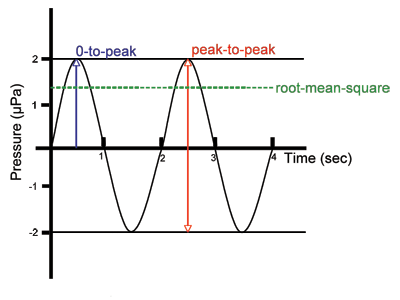
\includegraphics[width=\linewidth]{analog_signal}
  \caption{Señal analógica que representa una onda sonora bajo el mar. Se muestran tres formas de caracterizar su intensidad: Valor de cero a pico, valor de pico a pico y raíz cuadrada del valor medio.}\label{fig:analog_signal}
  
\endminipage\hfill
\end{figure}

\item Señal digital
\\
Se puede partir de una señal analógica senoidal y entonces llegar a una señal discretizada tomando valores equidistantes en el tiempo.

Para obtener una señal digital, se codifican cada uno de los valores discretos de la señal representada anteriormente. De este modo se tiene un número finito de valores pertenecientes a un conjunto.

Se aprecia en la figura \ref{fig:adc} el funcionamiento básico de un convertidor analógico/digital para comprender la diferencia entre estos dos conceptos.

\begin{figure}[!htb]
\centering
\minipage{0.7\textwidth}
  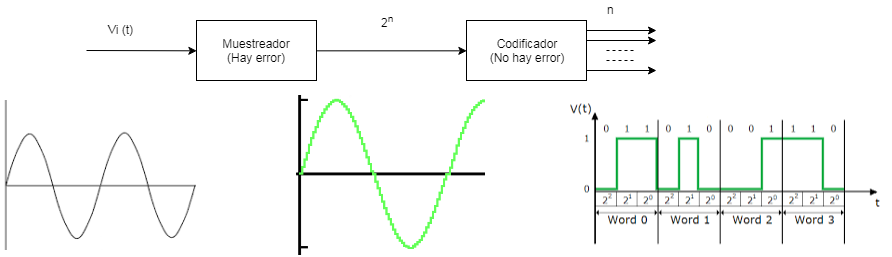
\includegraphics[width=\linewidth]{adc}
  \caption{Convertidor analógico-digital. La señal digital resultante forma palabras con  bits, es decir, se tienen en total $2^3=8$  valores diferentes y únicos.}\label{fig:adc}
\endminipage\hfill
\end{figure}


\end{itemize}

Volviendo al enfrentamiento entre el funcionamiento de la visión humana y artificial, se establece la comparación de ambas a continuación:

\begin{itemize}
\item Ojo humano
\\
Por una parte el ser humano recibe información visual tal y como se describiría en un mundo analógico,es decir, de forma continua.
\\
Sin entrar en demasiado detalle en el ámbito anatómico, la visión en el hombre se explica como la capacidad del ojo para detectar la luz y transformar la energía lumínica en señales eléctricas las cuales viajan al cerebro mediante el nervio óptico. Entre sus componentes principales se encuentran la córnea, la parte más externa del ojo, el cristalino, una lente ajustable según la distancia al objetivo así como un ``diafragma'' denominado pupila, cuyo diámetro está regulado por el iris, y la retina que se trata del tejido sensible a la luz. 

El funcionamiento del ojo se explica\cite{ojo_humano} porque la luz es refractada por la córnea al atravesarla. Esta luz refractada pasa a través de la pupila y el cristalino y se proyecta sobre la retina, zona en la que unas células fotorreceptoras la transforman en impulsos nerviosos que se trasladan, a través del nervio óptico, al cerebro.

%https://steemit.com/science/@greenrun/the-human-eye-and-vision-a-fascinating-phenomenon

\begin{figure}[!htb]
\centering
\minipage{0.50\textwidth}
  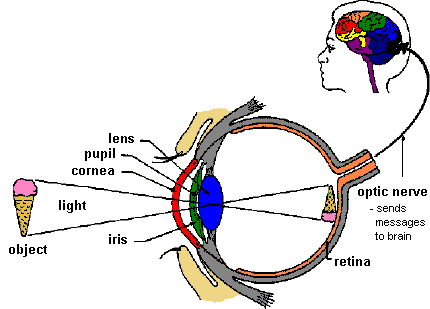
\includegraphics[width=\linewidth]{human_vision}
  \caption{Esquema del proceso de adquisición de información visual a través del ojo.}\label{fig:human_vision}
\endminipage\hfill
\end{figure}

Se ve claramente un tipo de señal analógica presente en el proceso, la luz, o mejor dicho la intensidad de la misma que pude representarse por la luminancia $L_v$, es decir, candela por metro cuadrado $\frac{cd}{m^2}$.

%https://es.wikipedia.org/wiki/Intensidad_luminosa
%https://es.wikipedia.org/wiki/Ojo_humano#Examen_del_ojo

\item Sensor artificial
\\
No se puede aplicar de forma directa el concepto del funcionamiento del ojo humano en un sensor artificial ya que necesita captar información analógica y digitalizarla para trabajar con ella.

De este modo hace falta unos pasos intermedios antes de llegar a un resultado final. Por lo tanto, hay que utilizar una aproximación diferente para resolver el problema y es aquí donde entra el concepto de nube de puntos. 
\end{itemize}

\fi

\section{Concepto de nube de puntos}\label{section:nubes_ejemplo}
Una nube de puntos se puede definir como una estructura $P$ que representa un conjunto de puntos multidimensionales $p \subset R_{n}$. En el caso de una nube de puntos en tres dimensiones, es decir $n=3$, cada elemento o punto está representado como mínimo por sus coordenadas geométricas $X,Y, Z$ respecto a un sistema de referencia conocido. Pero se pueden añadir más datos todavía en forma de color, curvatura o información sobre la normal $\vec{n}$ a una superficie en un ámbito local de la misma.  
\\
\\
Por lo tanto una nube de puntos\cite{point_cloud} es un conjunto desestructurado de puntos individuales sin relación alguna entre ellos, cuya
posición, color\cite{point_cloud_rgb} y otro tipo de características tienen definición, edición y representación muy simple. Esto implica que sea realmente práctico y sencillo manejar una gran cantidad de puntos sin tener que preocuparse por
conceptos como escala, rotaciones y demás relaciones entre diferentes puntos de un mismo objeto, siempre y cuando se tome la consideración más básica de la idea de nube de puntos.
\\
\\
%https://www.3deling.com/whta-is-a-point-cloud/
%https://www.3deling.com/rgb-point-cloud/
Se puede derivar de este concepto una gran potencia y flexibilidad ya que si se tienen una cantidad
suficiente de puntos dispuestos correctamente se pueden representar todo tipo de superficies aunque en
realidad no se trate de un plano continuo, es decir, el cerebro es capaz de interpretar complejas formas a
partir de información puntual en el espacio. Es más, se pueden llevar a cabo conversiones para relacionar el conjunto de puntos de la nube y crear
superficies reales en tres dimensiones. Este tipo de conversión se denomina también como reconstrucción de superficies, es decir, se parte de información puntual y se crea una superficie continua estimando qué
relación puede haber entre puntos cercanos. De esta forma, una nube de puntos puede transformarse a una
malla de polígonos o triángulos o incluso modelos CAD.
\\
\\
Las técnicas de reconstrucción de superficies son variadas y entre ellas se encuentran la triangulación de
Delaunay, que construye una red de triángulos sobre los vértices de la nube de puntos y la cual establece que:
\\
\\
\textit{``La circunferencia circunscrita de un triángulo no debe contener ningún otro vértice de la triangulación en su interior, admitiéndose vértices situados sobre la circunferencia.''}
\\
\\
En este contexto ``vértice'' se entiende por un punto de la nube de puntos.
Por lo tanto una red de triángulos es una triangulación de Delaunay si todos y cada uno de los triángulos que la forman cumplen la condición descrita que puede aplicarse tanto en espacios bidimensionales como tridimensionales. La apreciación gráfica del mencionado concepto puede verse en las figuras \ref{fig:del_mal}, \ref{fig:del_bien} y \ref{fig:del_bien_10pts}.
\\
\\
\begin{figure}[!htb]
\minipage{0.32\textwidth}
  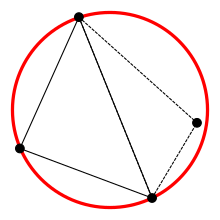
\includegraphics[scale=0.55]{delaunay_mal} 
\caption{Vértice en el interior de una circunferencia circunscrita. No se cumple la condición de Delaunay.}
\label{fig:del_mal}
\endminipage\hfill
\minipage{0.32\textwidth}
 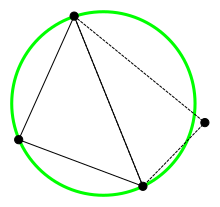
\includegraphics[scale=0.55]{delaunay_bien}
\caption{Vértice fuera de una circunferencia circunscrita. Se cumple la condición de Delaunay.}
\label{fig:del_bien}
\endminipage\hfill
\minipage{0.32\textwidth}
  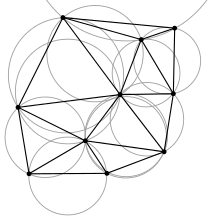
\includegraphics[scale=0.55]{delaunay_bien_10pts}
\caption{Triangulación de Delaunay aplicada a 10 puntos. Ninguna de las circunferencias circunscritas contiene vértices en su interior.}
\label{fig:del_bien_10pts}
\endminipage\hfill
\end{figure}
Por otra parte, una peculiaridad o limitación respecto a las nubes de puntos tiene que ver con que la
información que representan es superficial, es decir, los puntos siempre pertenecen a la superficie del
objeto en cuestión ya que es el lugar donde la luz de los escáneres llega, rebota y devuelve la
información correspondiente, proceso que se explica con más profundidad en apartados posteriores.
\\
Otra desventaja inherente a las nubes de puntos es la interpretación de la información que contienen ya
que se ha explicado que está compuesta de un conjunto de objetos o puntos sin relación entre ellos lo que dificulta la automotización de tareas tales como el reconocimiento y seguimiento de objetos mediante máquinas o identificación de formas y patrones. Es
aquí donde se requiere intervención del ser humano pues es su cerebro el que puede encontrar la similitud
entre una nube de puntos dada y el objeto o escenario que se supone que representa. Existen algoritmos capaces
de encontrar patrones y características para clasificar nubes de puntos pero nunca de forma
completamente fiable.

\subsection*{Ejemplos de nubes de puntos}
Habiendo tratado ya la teoría que rodea a la idea de ``nube de puntos'', se van a plantear a continuación diferentes ejemplos para apreciar la variedad y versatilidad que ofrecen.
\\
\\
En primer lugar se tiene en la figura \ref{fig:bunny_simple} una sencilla nube de puntos que representa un conejo. Se ha tomado una captura desde uno de todos los posibles puntos de vista que ofrece una visión en 360º.
Un ejemplo algo más elaborado se recoge en la figura \ref{fig:wolf} en la que aparece una nube que representa un lobo. 
Otro ejemplo de mayor complejidad permite observar en la figura \ref{fig:botes_grande} un escaneo frontal de tres botes de plástico. En este caso, es obvio que las zonas vacías justo detrás de los botes son aquellos lugares donde los rayos de luz emitidos por el sensor no pueden llegar ya que los propios botes los bloquean lo cual sirve para que su superficie quede capturada. Además, se ha incluido un campo de color para cada punto.
\\
\\
\begin{figure}[!htb]
\minipage{0.48\textwidth}
  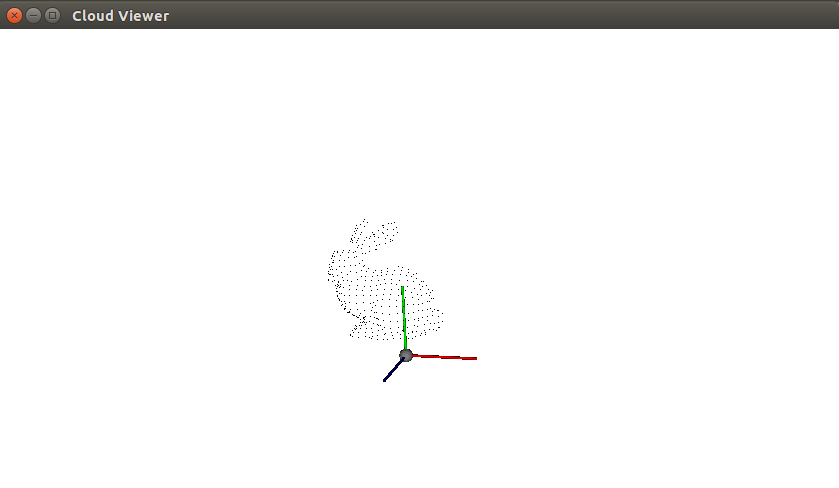
\includegraphics[scale=0.35]{bunny_simple}
  \caption{Nube de puntos representando un conejo.
  Peso total de la nube: 10.6KB.
  Número total de puntos: 397.}\label{fig:bunny_simple}
\endminipage\hfill
\minipage{0.48\textwidth}
  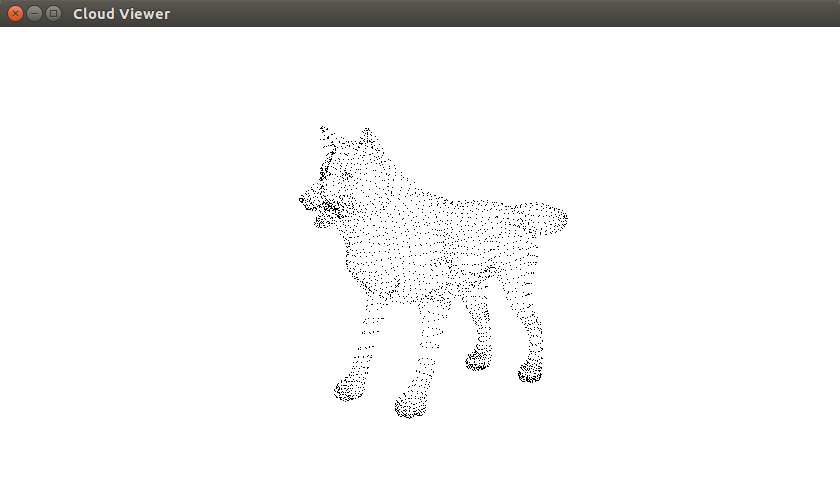
\includegraphics[scale=0.35]{wolf}
  \caption{Nube de puntos representando un lobo.
  Peso total de la nube: 42.6KB.
  Número total de puntos: 3400.}\label{fig:wolf}
\endminipage\hfill
\end{figure}

\begin{figure}
\centering
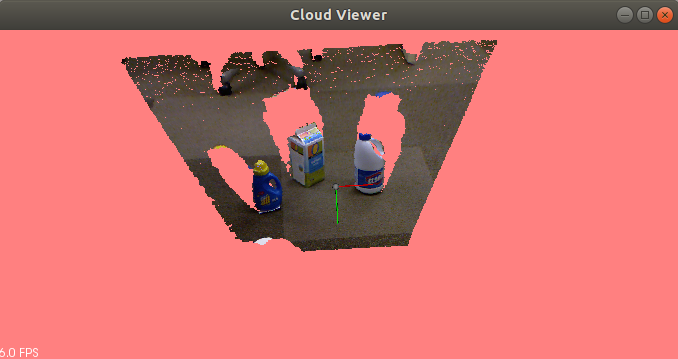
\includegraphics[scale=0.6]{botes}
  \caption{Nube de puntos representando tres botes.
  Peso total de la nube: 2.43MB.
  Número total de puntos: 307200.}\label{fig:botes_grande}
\end{figure}
%http://www.pointclouds.org/news/2013/01/07/point-cloud-data-sets/
%https://www.cc.gatech.edu/~turk/bunny/bunny.html
Una vez vistos ejemplos de nubes de puntos con la información suficiente para reconocer qué objeto representan sin más ayuda que la de los propios ojos, es momento de subir el nivel de complejidad para dar lugar a nubes de puntos más elaboradas y complejas. Se ha visto anteriormente una sencilla representación de un conejo con solamente 397 puntos. El nivel de detalle puede incrementarse a niveles del orden de decenas de miles de puntos tal y como es el caso de la figura \ref{fig:bunny} que representa un conejo de arcilla\cite{pcl_conejo_stanford} de 7.5 pulgadas de alto con unos 69451 triángulos ya que se ha llevado a cabo la reconstrucción de la superficie. Además, en la figura \ref{fig:bunny_colored} se aprecia el resultado si se añade información sobre color en cada punto. Como consecuencia de añadir más información (más de 90 veces la cantidad de puntos y el color) se tiene en este caso un peso de 22MB y hasta 35947 puntos.
\\
%http://graphics.stanford.edu/data/3Dscanrep/
\begin{figure}[!htb]
\minipage{0.45\textwidth}
  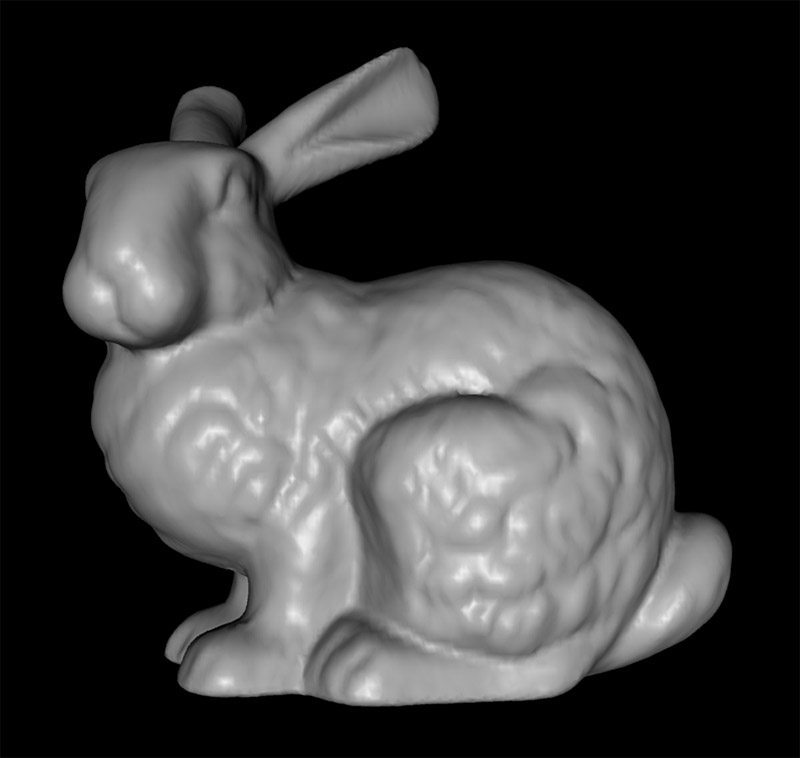
\includegraphics[width=\linewidth]{bunny}
  \caption{Nube de puntos con reconstrucción de superficie representando un conejo sin información de color.}\label{fig:bunny}
\endminipage\hfill
\minipage{0.45\textwidth}
  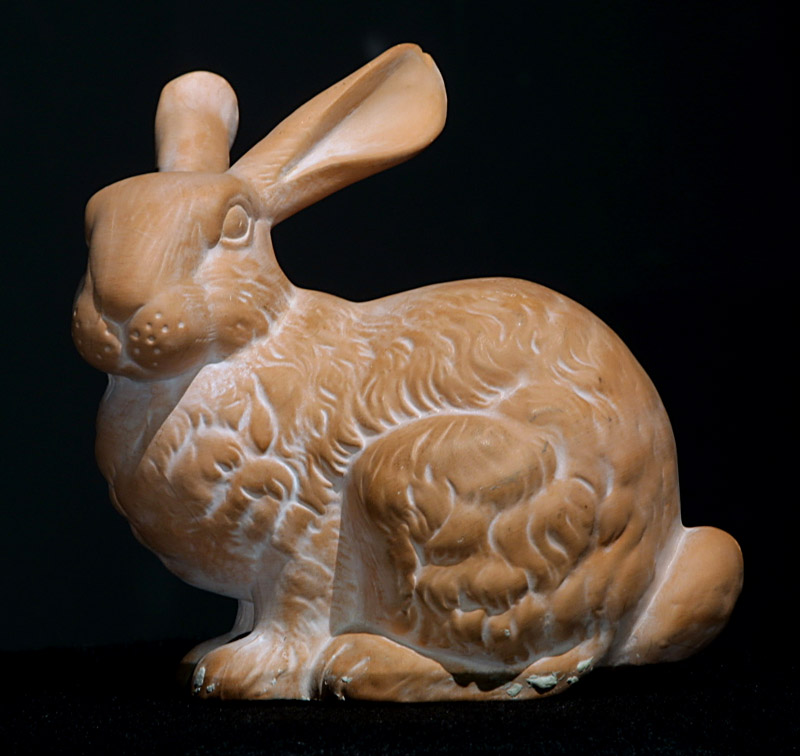
\includegraphics[width=\linewidth]{bunny_colored}
  \caption{Nube de puntos con reconstrucción de superficie representando un conejo con información de color.}\label{fig:bunny_colored}
\endminipage\hfill
\end{figure}
Esta nube de puntos proviene del departamento de computación gráfica de la universidad de Stanford e hicieron falta un total de 10 escaneos con el escaner Cyberware 3030 MS\cite{escaner_cyberware} para llegar al resultado final. Para hacerse una idea del tipo de sensor utilizado, se tiene como dato relevante su precio de unos 10000 dólares teniendo en cuenta además de que se trata de un sensor antiguo pues el escaneo se produjo en 1993.
\\
\\
Otro objeto de elevada complejidad que ha sido escaneado en las mismas condiciones que el mencionado conejo es el ángel Lucy\cite{pcl_conejo_stanford} mostrado en la figura \ref{fig:angel_lucy}. Un total de 47 escaneos dan lugar a un resultado final de 14027932 puntos y 28055742 triángulos y para este caso un peso de 508MB tomando la nube de puntos reconstruida y descomprimida.
\\
\\
\begin{figure}
\centering
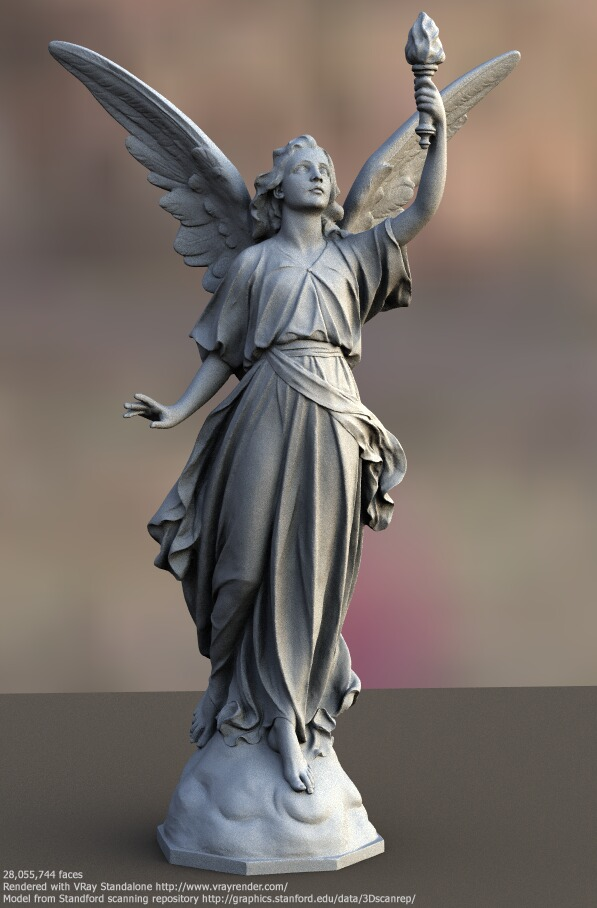
\includegraphics[scale=0.27]{angel_lucy}
\caption{Nube de puntos con reconstrucción de superficie representando una figura de un ángel.}\label{fig:angel_lucy}
\end{figure}
Pero no solamente se pueden representar objetos mediante nubes de puntos sino entornos abiertos o interiores. Johannes Schauer y Andreas Nüchter de la universidad de Würzburg, Alemania, tomaron una nube de puntos\cite{pcd_exteriores} del mercado en la ciudad de Würzburg tal y como se ve en la figura \ref{fig:wue_city}.
El escaner utilizado en el este caso es el Riegl VZ-400\cite{escaner_riegl} y con un total de 6 escaneos se han conseguido 86585411 puntos conteniendo cada uno de ellos información sobre la reflectancia de la luz del sensor lo que se aprecia con puntos de diferente claridad ya que no hay información sobre color. Obviamente, un entorno exterior contiene mucha más información que un simple objeto por lo que esta nube de puntos tiene un peso de 5117MB descomprimida. Cabe destacar que el sensor utilizado es bastante más potente que el anteriormente mencionado y tiene un precio de unos 80000 dólares.
\\
\\
%http://kos.informatik.uni-osnabrueck.de/3Dscans/
%http://www.riegl.com/uploads/tx_pxpriegldownloads/10_DataSheet_VZ-400_2017-06-14.pdf
%https://www.microgeo.it/es/esc%C3%A0ner-l%C3%A0ser-3d/modelos/scanner-riegl-vz400.aspx
\begin{figure}
\centering
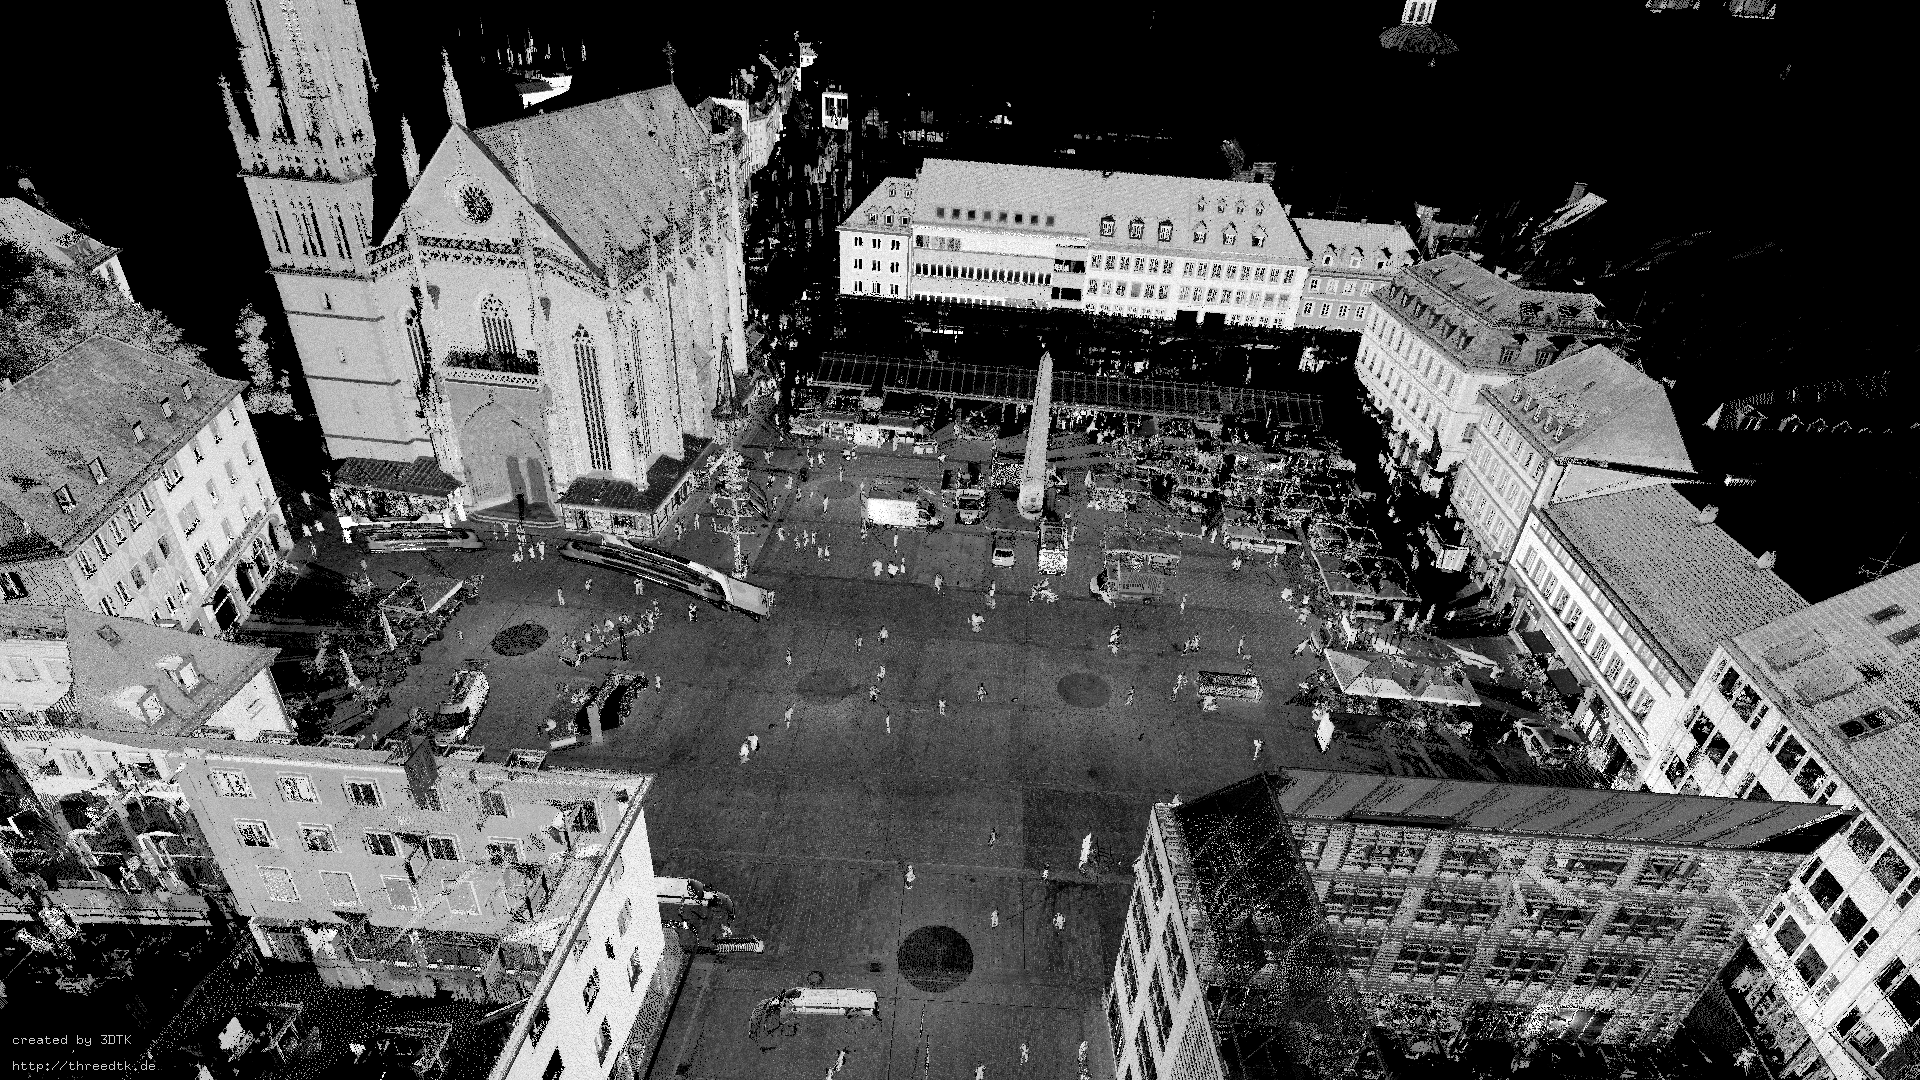
\includegraphics[scale=0.17]{wue_city2}
\caption{Nube de puntos con información de reflectancia de la luz que representa un mercado en Würzburg, Alemania.}\label{fig:wue_city}
\end{figure}
Por último, Dorit Borrmann obtuvo una nube de puntos\cite{pcd_exteriores} mostrada en la figura \ref{fig:joined_model} que representa el interior del laboratorio de automática en la universidad de Jacobs, Bremen. Se pueden apreciar diferentes tipos de puntos para cada sección de la imagen ya que el sensor láser Riegl VZ-400 se encarga de representar información térmica y de profundidad mientras que las cámaras Optris PI IR y Logitech QuickCam 9000 Pro muestran información relacionada con el color. Se hicieron un total de 9 escaneos en 40º cada uno lo que permite disponer de una imagen en 360º (la imagen mostrada es uno de los escaneos)
\\
\\
\begin{figure}
\centering
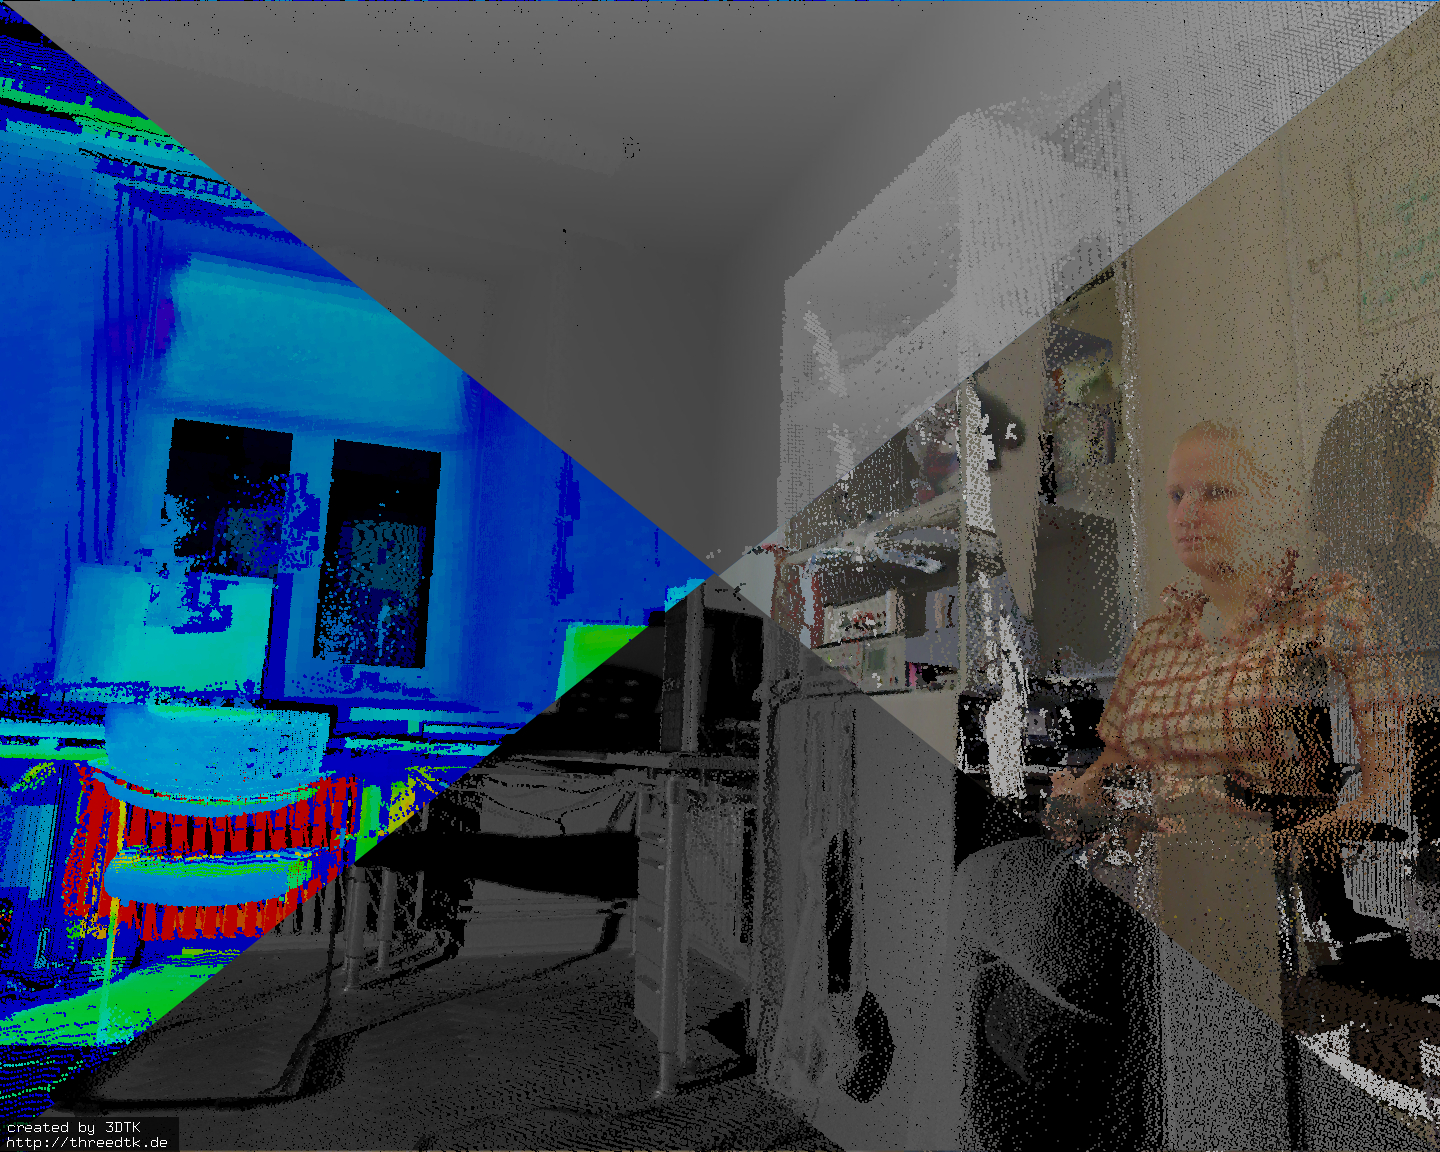
\includegraphics[scale=0.17]{joinedmodel}
\caption{Unión de cuatro nubes de puntos con información térmica, de color y reflectancia de la luz representando un entorno cerrado.}\label{fig:joined_model}
\end{figure}


Se han visto varios ejemplos que muestran la potencia del concepto de nube de puntos y es ahora el momento de conocer cómo se ha transformado una porción de la realidad en un conjunto de puntos que la representan.
\section{Sensores para captura de nubes de puntos}
La adquisición y almacenamiento de información es el primer paso para comenzar a trabajar con una nube de puntos. A pesar de tratarse de información relativamente sencilla como coordenadas respecto a un sistema de referencia, color y reflectividad, hay que tomar dicha información para miles o incluso millones de puntos tal y como se ha visto en ejemplos mostrados anteriormente como en el caso del ángel Lucy de la figura \ref{fig:angel_lucy}. 
\\
\\
En los últimos veinte años, se han hecho grandes progresos en lo que a sensores se refiere ya que actualmente se usan de sofisticadas cámaras y escaneres láser y se han dejado atrás los sensores basados en sonar o infrarrojos los cuales proporcionan a penas unos bytes de información sobre el entorno u objeto que tratan de representar.
\\
\\
Existen dos métodos para generar nubes de puntos tridimensionales: escaneo en tres dimensiones con un láser y fotogrametría.

\subsection{Escaneo en tres dimensiones: LIDAR}
Centrándose en los sensores láser, la adquisición de información cobra sentido cuando se estudia el comportamiento de los rayos de luz ya sea visible o infrarroja, por ejemplo. Para poder llevar a cabo el escaneo de objetos tridimensionales así como entornos, se usa el escaneo láser o también conocido como Light Detection And Ranging (LIDAR)\cite{lidar},originalmente se conocía por la unión de ``light'' ``radar'', 
procedimiento que se originó a principios de la década de los sesenta tras la invención del láser y que permite medir distancias a un objetivo iluminándolo con pulsos de luz.
\\
\\
Pero, ¿Cómo se pueden medir distancias utilizando luz? el concepto entorno al que el escáner láser gira es el tiempo de vuelo. Esto quiere decir que se utiliza un dispositivo conocido como ``range finder'' capaz de medir con precisión el tiempo que transcurre desde que se emite un pulso de luz hasta que vuelve otra vez al mismo tras rebotar sobre el objeto que desea detectarse. Considerando entonces $c$ constante conocida que representa la velocidad de la luz, la distancia del escáner a un punto en concreto donde rebota un determinado pulso de luz puede determinarse como:

$$d = \frac{c*t}{2}$$

Nótese que $c*t$ es la distancia que hay entre el escaner y el objeto duplicada ya que $t$ es el tiempo total desde la emisión del pulso de luz hasta la recepción. Por tanto, tomando la mitad del tiempo total de vuelo se obtiene la medida deseada que es la distancia del escáner al objeto.

\begin{figure}
\centering
\minipage{0.6\textwidth}
  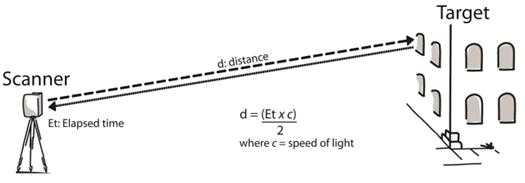
\includegraphics[width=\linewidth]{lidar_explanation}
  \caption{Ejemplo ilustrativo de medición de distancia de un sensor lidar a un edificio}\label{fig:lidar explanation}
\endminipage\hfill

\end{figure}

\iffalse
Para cada pulso de luz emitido se detecta un punto en concreto lo que hace pensar que para poder crear nubes con millones de puntos la velocidad de generación de los pulsos ha de ser elevada. En el caso de lidar se pueden emitir hasta 150000 pulsos en un segundo.
\\
\\
De este modo, al ser capaz de medir la distancia que hay desde el punto de emisión de los rayos de luz hasta la superficie en la que rebotan, el sensor puede detectar rápidamente formas definidas de objetos, edificios o paisajes considerando en conjunto de puntos detectados tal y como se ha mostrado en ejemplos del apartado \ref{section:nubes_ejemplo}
\fi
\subsubsection{Control de la luz utilizada por el sensor}
\iffalse
El componente esencial en un sistema LIDAR es el rayo de luz que permite hacer las mediciones. Por lo general, hay dos tipos de LIDAR:
método coherente e incoherente o también conocido como detección de energía directa.
\\
El método incoherente mide cambios en la amplitud de la onda emitida pues al rebotar con los objetos su nivel de energía varía.
El método coherente es más apropiado para medir diferencias en la frecuencia de la onda y utiliza modulación en fase y/o frecuencia de la misma lo que le permite operar a potencias mucho más bajas a costa de utilizar un equipamiento más complejo.
\\
\\
En ambos modelos se pueden usar dos tipos diferentes de pulsos: micropulsos y sistemas de alta energía.
\\
los micropulsos surgen de la elevada capacidad computacional de las computadoras actuales. Esto deriva en un láser de baja potencia (del orden del $\mu$J) que es clasificado como seguro al ojo permitiéndose su uso bajo escasas medidas de precaución.
\\
Por otra parte, los sistemas de alta energía, requieren medidas de seguridad más estrictas y se usan principalmente para fines de investigación atmosférica pues permite tomar medidas como la altura, número de capas y densidad de las nubes, propiedades de las partículas en las nubes, temperatura, presión, concentración de gases, o humedad.
\\
\\
\fi
En cuanto al control del láser\cite{control_laser}, en la mayoría de los escaneres, la dirección de emisión del rayo de luz es constante por lo que para poder apuntar el haz hacia la dirección deseada se hace uso de espejos. Esto implica lanzar el láser contra un espejo y controlar éste con diferentes movimientos de rotación; en un eje para un movimiento unidimensional (un grado de libertad) o en dos ejes para un alcance espacial total quedando fija la posición del foco emisor (dos grados de libertad)

\begin{figure}[!htb]
\minipage{0.32\textwidth}
  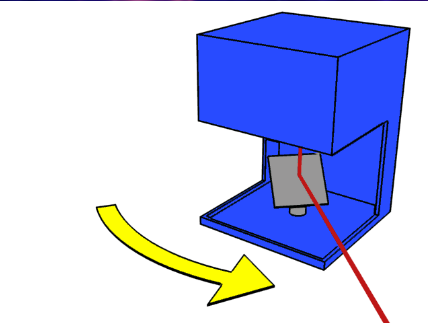
\includegraphics[width=\linewidth]{sensor_laser_espejo}
  \caption{Láser proyectado contra un espejo con un grado de libertad.}\label{fig:sensor laser completo - espejo}
\endminipage\hfill
\minipage{0.32\textwidth}
  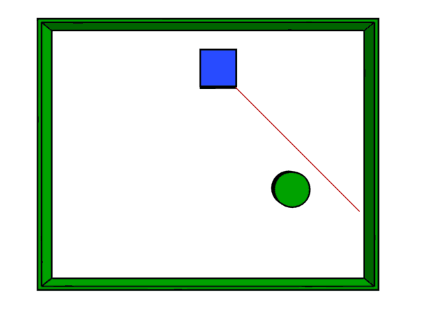
\includegraphics[width=\linewidth]{sensor_laser_vista_tope}
  \caption{Vista superior del sensor y las superficies que obstaculizan el haz de luz: objeto y recinto en el que se encuentra.}\label{fig:sensor laser completo - vista tope}
\endminipage\hfill
\minipage{0.32\textwidth}
  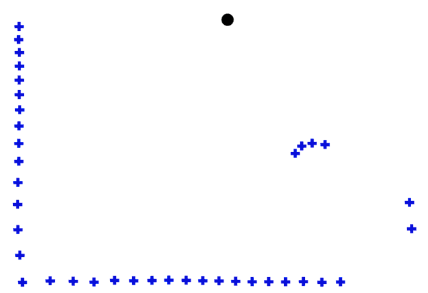
\includegraphics[width=\linewidth]{sensor_laser_resultado}
  \caption{Conjunto de puntos obtenidos tras el esacaneo pertenecientes al objeto en el interior del recinto y las limitaciones espaciales del mismo.}\label{fig:sensor laser completo - resultado}
\endminipage
\end{figure}

Una alternativa para controlar el rayo láser en dos dimensiones incumbe el uso de dos espejos montados en ejes ortogonales y entonces hacer movimientos de rotación entorno a un eje para cada uno de los espejos.

\begin{figure}
\minipage{0.45\textwidth}
  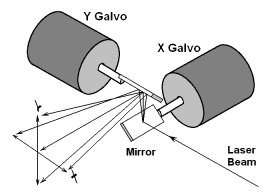
\includegraphics[width=\linewidth]{sensor_dos_espejos}
  \caption{Uso de dos espejos con un grado de libertad en cada uno y accionados con galvanómetros}\label{fig:sensor dos espejos}
\endminipage\hfill
\minipage{0.45\textwidth}
  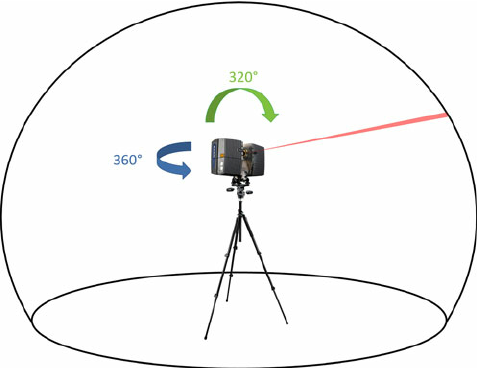
\includegraphics[width=\linewidth]{movimiento_lidar_2D}
  \caption{Sensor lidar con dos grados de libertad.}\label{fig:movimiento lidar 2D}
\endminipage\hfill

\end{figure}

Para sistemas más sofisticados todavía, se requiere el posicionamiento espacial del foco emisor de rayos lo cual se consigue con un sistema de lentes servo controladas conocido como focus shifter o z-shifter.
\\
\\
La forma más común de mover los espejos es mediante el uso de un motor eléctrico o un galvanómetro para el más sencillo de los casos. Se pueden utilizar también actuadores piezoeléctricos o magnetorresistivos para una mayor velocidad angular pero a costa de menores ángulos máximos de desplazamiento.

\iffalse
\subsubsection{Ventajas y desventajas de LIDAR}

Retomando la idea de que la velocidad de la luz es una constante, la única variable en el cálculo de la distancia es el tiempo de vuelo. Téngase por ejemplo una distancia de 30cm desde el sensor hasta el objeto que desea capturarse. Esto implica que la resolución del reloj integrado en el sensor ha de ser cuanto menos elevada:

\begin{equation}
\frac{0.3m}{3*10^{8}\frac{m}{s}} = 1ns =0,000000001s
\end{equation}

Se ha desvelado de esta forma una desventaja del concepto de tiempo de vuelo, se necesita equipamiento muy preciso y de elevada repetibilidad lo que se traduce en complejidad y elevadas inversiones económicas.
\\
\\
Pero dando la vuelta a esta desventaja, es decir, cuando se trata de escanear objetos en la lejanía como puede ser un edificio o paisaje, la resolución requerida por parte del reloj se reduce dando así medidas más fiables. Además, considerando de nuevo la velocidad de la luz como una constante, no importa la distancia a la que se encuentre el objeto salvo por cuestiones de difracción y absorción del pulso de luz en el ambiente, por ejemplo, por la presencia de humedad.
\\
\\
Por lo tanto, el método LIDAR combina precisión y versatilidad ya que puede valerse de luz visible, infrarroja o ultravioleta para lanzarla contra objetivos de diversos tipos de materiales como metal, cerámica, aerosoles, terreno (rocas y tierra) e incluso se puede llegar al nivel molecular. 
\\
\\    
Sin embargo no se realiza un único escaneo ya que el propio concepto implica que el objeto bloquea los rayos de luz por lo que la cara frontal, de la que sí se obtiene información, impide a la luz llegar a la cara posterior. El factor clave es entonces el hecho de que estos rayos de luz puedan llegar a toda la superficie del objeto que se quiere analizar, es decir, accesibilidad física del sensor.
De este modo, independientemente del sensor o método que se utilice, es imposible recolectar
información sobre superficies no visibles o lo que es lo mismo, con un solo escaneo.
\\
Este efecto puede apreciarse en la figura \ref{fig:botes_grande} donde falta información en el seno de la nube de puntos en forma de tres áreas en las que no hay ningún punto pues son la ``sombra'' de los botes ante los rayos de luz del escaner.
\\
Como consecuencia, es necesario llevar a cabo varios escaneos desde diferentes puntos de vista y
ponerlos en conjunto conociendo con precisión la posición del sensor en cada escaneo para poder llevar a cabo lo que se conoce como alineamiento de nubes de puntos, concepto que se explicará con más detalle posteriormente.
\fi


\iffalse
\subsubsection{Alternativas a LIDAR}

Disponer de complejas, fiables y robustas representaciones del mundo real tiene no es tan sencillo como pueda parecer puesto que estos sensores suelen tener un precio prohibitivo para la mayoría de los interesados ya sean particulares o incluso empresas con un poder adquisitivo considerable. Véanse por ejemplo los sensores mencionados en el apartado \ref{section:nubes_ejemplo} los cuales tienen un precio de más de 70000\$.

Sin embargo, la situación ha cambiado desde que han aparecido en el mercado ciertos sensores 3D como por ejemplo el sensor Kinect de la consola Xbox360 de Microsoft\cite{kinect}. Aunque este sensor puede trabajar con nubes de puntos en tiempo real e imágenes en 2D su precio no supera los 150\$. De este modo se ha producido un gran paso adelante en cuanto a los impedimentos relacionados con la adquisición, mantenimiento y delicadeza del hardware que traduce el mundo real a nubes de puntos.

%https://www.matec-conferences.org/articles/matecconf/pdf/2018/32/matecconf_smima2018_03001.pdf
%https://erget.wordpress.com/2014/04/27/producing-3d-point-clouds-with-a-stereo-camera-in-opencv/
\fi
\subsection{Fotogrametría}
En el caso de la fotogrametría\cite{fotogrametria}, la información tridimensional se obtiene a partir de la triangulación efectuada sobre fotografías en dos dimensiones tomadas al objeto desde diferentes posiciones ya conocidas.

Hay una serie de pasos genéricos para obtener nubes de puntos a partir de fotografías en dos dimensiones:
\begin{itemize}
\item[•] Detección de puntos clave, es decir, puntos invariantes a la escala y rotación que pueden ser utilizados para alinear el conjunto de fotos y dar sentido tridimensional.
\item[•] Emparejamiento de puntos clave de las diferentes fotos tomadas.
\item[•] Alineamiento de cámaras: se calcula la distancia de las cámaras a los puntos claves minimizando el error entre las distancias en las imágenes y las distancias esperadas para cada cámara.
\item[•] Construcción de la nube de puntos: se crea una nube de puntos densa (ningún punto se sitúa en el infinito o está indeterminado) una vez se tienen las cámaras alineadas y se conocen las distancias entre los puntos clave. Este proceso es el de mayor carga computacional.
\end{itemize}

Como ejemplo, se muestra en la figura \ref{fig:cloud_photo} el resultado de aplicar este método sobre un jaguar tipo e\cite{fotogrametria}. 
\begin{figure}
\centering
\minipage{0.7\textwidth}
  \includegraphics[width=\linewidth]{cloud_photo}
  \caption{Construcción de nube de puntos mediante fotogrametría. El cuadro rojo indica detección de falsos puntos clave debido a reflejos de la luz en el metal.}\label{fig:cloud_photo}
\endminipage\hfill
\end{figure}
Las fotografías fueron tomadas con una Canon 550d\cite{canon} la cual es fácilmente adquirible a minoristas. Para ello, se movió la cámara alrededor del vehículo y se tomaban las respectivas fotografías para capturar todos sus puntos clave. se repitió este proceso posicionando la cámara a diferentes alturas.
\\
\\
El software utilizado para procesar las fotografías y obtener la nube de puntos es Agisofts photoscan\cite{agisoft}, un software de fotogrametría comercial. Este software ofrece gran control al usuario sobre la nube de puntos final pues puede determinar parámetros como el tamaño de la nube y su formato. Además, Agisofts photoscan puede no solamente producir una red de triángulos a partir de la nube estimada y añadirle textura sino exportar la nube de puntos para que pueda ser procesada con otro software.



\subsubsection{Comparación entre LIDAR y fotogrametría}
La resolución alcanzada por el escaneo tridimensional es generalmente mayor que la obtenida con fotogrametría ya que ésta es resultado de operaciones sobre fotografías en dos dimensiones y el escaneo tridimensional aporta medidas directas.
\\
\\
Pero las desventajas del escaneo tridimensional respecto a la fotogrametría son notorias:
\begin{itemize}
\item[•] El equipo necesario es generalmente de alto coste y complejo de utilizar por lo que se requieren conocimientos adicionales. 
\item[•] El sensor adquiere todo tipo de información a su alcance, es decir, no criba información innecesaria o ruido, por lo que se captura una gran cantidad de puntos lo que implica elevados tiempos para el posterior procesamiento de la nube.
\item[•] Los sensores pueden llegar a tardar días en generar nubes de puntos de objetos o entornos muy grandes.
\end{itemize}   


%REFERENCIA paper de catpuras de nubes en documentacion

Por lo tanto, para escaneos sencillos y que no requieran elevada resolución, es más ventajoso utilizar fotogrametría porque es suficiente con una cámara digital convencional, no se requieren conocimientos sobre sensores láser, el procesamiento es más liviano porque se capturan menos puntos y el proceso de captura es mucho más rápido.

\subsection{Aplicaciones potenciales de nubes de puntos}
\subsubsection{Reconocimiento de terreno}
Una aplicación muy extendida de LIDAR es el reconocimiento de terreno. Para ello se integra el sensor en una aeronave y se capturan los puntos correspondientes al terreno sobrevolado. Esta aplicación es útil para generar modelos digitales de elevación.
\\
\\
Como contrapartida, hay que tener en cuenta que el sensor tiene una posición variable respecto al terreno ya que va embarcado en una aeronave. Para considerar esto en el resultado final de la nube de puntos generada, se ha de disponer de un sistema de navegación, para el posicionamiento del sensor con GPS por ejemplo, así como de una Intertial Measurement Unit (IMU) o unidad de medidas inerciales para obtener información sobre la orientación absoluta del sensor.

 
\begin{figure}
\minipage{0.45\textwidth}
  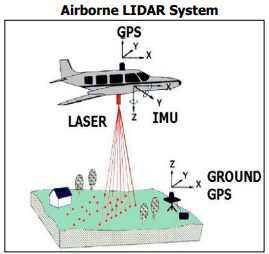
\includegraphics[width=\linewidth]{airborne_lidar}
  \caption{Esquema de utilización del método lidar en una aeroanve}\label{fig:airborne_lidar}
\endminipage\hfill
\minipage{0.45\textwidth}
  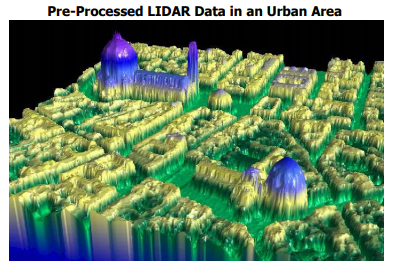
\includegraphics[width=\linewidth]{airborne_city}
  \caption{Entorno urbano recreado con el método lidar}\label{fig:airborne_city}
\endminipage\hfill

\end{figure}


%https://upload.wikimedia.org/wikipedia/commons/c/c0/LIDAR-scanned-SICK-LMS-animation.gif

%https://www.engineering.com/AdvancedManufacturing/ArticleID/12390/Quality-Basics-How-Does-3D-Laser-Scanning-Work.aspx

%https://en.wikipedia.org/wiki/Laser_scanning

%http://www.2grobotics.com/wp-content/uploads/2017/03/sonarvslaser.pdf

%http://www.lidar-uk.com/how-lidar-works/

%http://elm-chan.org/works/vlp/report_e.html
%http://www.ionix.fi/en/technologies/laser-processing/laser-marking/

\subsubsection{Vehículos autónomos}
Los vehículos autónomos ya existentes y del futuro no requieren ningún tipo de interacción humana durante el trayecto. Para conseguir este objetivo, es necesario controlar el comportamiento, posición y trayectoria del vehículo en todo momento así como tomar medidas del entorno constantemente lo cual requiere un uso redundante de sensores para obtener medidas de alta precisión y fiabilidad.
\\
\\
Por lo tanto, un vehículo autónomo no debe ignorar técnicas de posicionamiento simultáneas lo que significa que las tradicionales que ya utiliza, posicionamiento por satélite (GNSS del inglés Global Navigation Satellite System o navegación global por satélite) y medidas inerciales (IMU del inglés Inertial Measurement Unit o unidad de medidas inerciales) deben poder ser extendidas con nuevas soluciones.
\\
\\
Una nueva solución puede basarse en el escaneo del entorno con cámaras y escáneres láser (LIDAR) De este modo, las mediciones efectuadas por la cámara y el sensor láser deben ser comparadas con una representación tridimensional de su entorno, algo semejante a un mapa que almacena información sobre la superficie de la carretera, objetos a su alrededor, los edificios cercanos, personas y cualquier otro elemento que influya en la navegación.
\\
\\
En el trabajo realizado por Vivien Potó, József Árpád Somogyi, Tamás Lovas, Árpád Barsi\cite{vehiculos_autonomos} de la universidad de tecnología y economía de Budapest, se puede apreciar el escaneo realizado sobre las calles Piarista y Váci. Para ello se utilizó el escáner láser Faro Focus 3D 120S\cite{faro} y el sistema de mapeado móvil Riegl VMX-450\cite{riegl_450}.
\\
\\
El escáner láser tiene un alcance máximo para tomar mediciones de 120m y puede generar 976000 puntos por segundo. Su ángulo de visión es de 360º horizontalmente y 305º en vertical. La resolución fue ajustada a 6mm a una distancia de 10m.
\\
\\
Para cubrir toda la calle, se realizaron 16 mediciones en total capturando por lo tanto más de 458 millones de puntos. En la figura \ref{fig:calles_budapest} se puede apreciar el fragmento de vía que fue escaneado y a partir del cual se generó la nube de puntos de la figura \ref{fig:calles_budapest_escaneo}

\begin{figure}[!htb]
\centering
\minipage{0.8\textwidth}
  \includegraphics[width=\linewidth]{calles_budapest}
  \caption{Calles Piarista y Váci siendo la línea roja el fragmento escaneado.}\label{fig:calles_budapest}
\endminipage\hfill

\end{figure}

\begin{figure}[!htb]
\centering
\minipage{0.8\textwidth}
  \includegraphics[width=\linewidth]{calles_budapest_escaneo}
  \caption{Nube depuntos generada a partir del escaneo de las calles Piarista y Váci}\label{fig:calles_budapest_escaneo}
\endminipage\hfill

\end{figure}

\section{Procesamiento software de nubes de puntos}\label{librerias}
Una vez se dispone de una nube de puntos, se precisa ahora de un mecanismo para trabajar con la información que hay en ella. El software existente para dicha tarea es diverso y no siempre gratuito. Como ejemplo se tiene RealityCapture\cite{realitycapture} o RC, un software capaz de crear modelos 3D a partir de fotografías o escaneos láser desordenados. Su alcance abarca aspectos como arte, arquitectura, escaneo completo del cuerpo humano, videojuegos, mapeado, efectos visuales y realidad virtual.
\\
Entre sus características se encuentran cálculo de redes de polígonos, coloreado, texturizado, georreferenciación, conversión de sistema de coordenadas, suavizado y operaciones de lectura/escritura de datos.
\\
\\
Existe más software semejante al descrito y la inmensa mayoría tiene limitaciones de licencias o de hardware demasiado potente, y por lo tanto de un valor económico elevado, ya no solamente para un usuario particular sino para muchas universidades y empresas. Pero entre todos ellos destaca PCL, siglas que en inglés se refieren a Point Cloud Library\cite{PCL}, es decir, ``librería de nubes de puntos'' y que está escrita en lenguaje C++. Es una librería única, de gran escala y un proyecto abierto a la comunidad para procesamiento de imágenes y nubes de puntos tanto en 2D como en 3D. Es más, PCL se somete a los términos de la licencia Berkeley Software Distribution (BSD) lo que implica que es de uso libre tanto para fines comerciales como de investigación. 
\begin{figure}
\centering
\minipage{0.45\textwidth}
  
\includegraphics[width=\linewidth]{pcl_logo}
  \caption{Logo de PCL}\label{fig:pcl logo}
\endminipage\hfill
\end{figure}
\\
\\
PCL dispone de multitud de herramientas para el procesamiento de nubes de puntos y dado que es una librería sometida a constante crecimiento y modificaciones, tener las herramientas debidamente organizadas y estructuradas es de vital importancia. Es por esto por lo que PCL tiene una organización en forma de módulos\cite{PCL_modulos}, es decir, el conjunto de herramientas se clasifica según su utilidad según la tabla \ref{tablaPCL}. Abordar en profundidad todos y cada uno de estos módulos conllevaría un trabajo demasiado extenso de modo que únicamente se entrará en detalle en aquellos que sean de utilidad para el propósito del presente trabajo y a lo cual se procede en el siguiente capítulo.
\begin{table}
\centering
\begin{tabular}{|L|c|L|}\hline
 \textbf{Nombre} & \textbf{Definición} \\\hline 
 
filters &  \multicolumn{1}{m{10cm}|}{Contiene mecanismos de eliminación de ruido y filtrado de puntos con determinadas características.}\\\hline

  features  & \multicolumn{1}{m{10cm}|}{Contiene estructuras de datos y mecanismos para estimación de características en 3D. Permiten detectar patrones geométricos haciendo uso de la información local que representa el entorno de un punto dentro de una nube.}\\\hline
  
  keypoints  & \multicolumn{1}{m{10cm}|}{Contiene las implementaciones de dos algoritmos de detección de keypoints (puntos clave) los cuales se explicarán detalladamente más adelante.}\\\hline
  
  registration  & \multicolumn{1}{m{10cm}|}{Permite unificar diferentes nubes de puntos en un modelo global y consistente. Se vale de los keypoints de cada uno de los conjuntos iniciales para poder desarrollar el modelo final unificado.}\\\hline
  
  kdtree  & \multicolumn{1}{m{10cm}|}{Proporciona estructuras de datos que particionan el espacio de trabajo para almacenar puntos en una estructura de árbol y así mejorar la eficiencia de las operaciones realizadas sobre la nube de puntos.}\\\hline
  
  octree  & \multicolumn{1}{m{10cm}|}{Proporciona métodos para crear estructuras de datos jerárquicas en forma de árbol para particionar el espacio de trabajo y agilizar futuras operaciones sobre la nube.}\\\hline
  
  segmentation  & \multicolumn{1}{m{10cm}|}{Contiene algoritmos para segmentar o dividir una nube en diferentes regiones. Su utilidad se revela al trabajar con nubes que constan de grupos aislados de puntos.}\\\hline
  
sample consensus  & \multicolumn{1}{m{10cm}|}{Contiene modelos de figuras geométricas predefinidas como líneas, planos o cilindros para detectar similitudes respecto a los mismos en una nube de puntos dada. Estos modelos se pueden combinar para dar lugar a una gran variedad de figuras geométricas.}\\\hline

  surface  & \multicolumn{1}{m{10cm}|}{Permite la reconstrucción de superficies sobre escaneos en 3D.}\\\hline
  
  recognition  & \multicolumn{1}{m{10cm}|}{Contiene algoritmos para el reconocimiento de diferentes tipos de objetos.}\\\hline
  
  io  & \multicolumn{1}{m{10cm}|}{Contiene clases y métodos para leer y escribir nubes de puntos en formato PCD que se explicará más adelante.}\\\hline
  
   visualization  & \multicolumn{1}{m{10cm}|}{Sirve para visualizar nubes de puntos y así apreciar los resultados de las operaciones realizadas sobre las mismas.}\\\hline
 
\end{tabular}\caption{Descripción de módulos de la librería PCL.}\label{tablaPCL}
\end{table}
\\
\\
A parte de los módulos o agrupaciones dentro de la librería de PCL, se requiere para su ejecución la instalación de una serie de librerías externas, que son:

\begin{itemize}
\item[•]Eigen\cite{eigen} Es una librería escrita en C++ para operaciones de álgebra lineal como operaciones con vectores, matrices o métodos numéricos.
\item[•]FLANN\cite{flann}: Son la siglas de Fast Library for Approximate Nearest Neighbors que se traduce como librería de aproximación rápida de vecinos más cercanos. Está escrita en C++ y sirve para realizar búsquedas rápidas de puntos vecinos cercanos a uno en concreto en espacios de diferentes dimensiones.
\item[•]boost\cite{boost}: Se trata de un conjunto de bibliotecas para extender las capacidades del lenguaje de programación C++ con funciones matemáticas y numéricas, de tratamiento de estructuras de datos y de entrada y salida, entre otras muchas.
\item[•]VTK\cite{vtk}: Son las siglas de Visualization Toolkit o kit de visualización. Está escrita en C++ y permite procesamiento y visualización de imágenes así como aporta soporte para multitud de algoritmos de visualización como es el escalar, vectorial, y métodos más avanzados como la triangulación de Delaunay.
\end{itemize}

\section{Capacidades de PCL}
\subsection{Módulo IO}
Uno de los módulos más importantes es el que se encarga de la lectura y escritura de nubes de puntos, es decir, el módulo IO del inglés input/output que se traduce como entrada/salida. Esta librería es capaz de interpretar la información otorgada por diferentes tipos de sensores así como de generar archivos que contienen nubes de puntos manipuladas por el resto de módulos.
\\
\\
PCL ha creado el formato PCD, del inglés Point Cloud Data, es decir ``datos de nube de puntos''. No se trata de un formato revolucionario sino más bien de una forma de complementar a los ya existentes que debido a los propósitos para los que se han creado u otras razones, no soportan algunas de las características relacionas con el procesamiento de nubes de puntos de $n$ dimensiones.
\\
\\
Un fichero PCD dispone de dos partes diferenciadas, encabezamiento y los puntos como tal. El encabezamiento se encarga de identificar y declarar las propiedades de la nube de puntos almacenados en el fichero y debe estar codificado en ASCII lo que implica que cada entrada en este formato está delimitada de las demás usando saltos de línea. Las características especificadas en el encabezamiento son las siguientes:
\begin{itemize}
\item VERSION:
Este campo especifica la versión del formato PCD

\item FIELDS:
Traducido como ``campos'' indica el nombre de cada dimensión o campo existente en la nube de puntos como por ejemplo color, coordenadas XYZ o normales a la superficie.

\item SIZE: 
Este campo indica el tamaño en bytes, y en el mismo orden, de cada campo declarado por FIELDS.

\item TYPE:
Representa el tipo de dato de cada campo con un carácter.\\ 
I: Tipos con signo como int8 que equivale a un char, int16 que equivale a un short y int32 que equivale a un int.\\
U: Tipos sin signo como uint8, uint16 y uint32, los tipos análogos al caso anterior pero sin signo.\\
F: Representa todos los tipos flotantes.

\item COUNT: 
Indica cuántos elementos tiene cada campo previamente declarado en FIELDS. Por defecto toma el valor de 1.

\item WIDTH:
Representa el ancho de la nube de puntos teniendo este concepto dos significados para lo cual hay que entender cómo se puede interpretar una nube de puntos. Por una parte, las nubes de puntos desorganizadas pueden verse como un vector de $n$ elementos donde $n$ es el ancho de la nube de puntos, es decir, se trata de una matriz de una fila y $n$ columnas donde $n$ es el ancho. Por otra parte, se puede definir de manera matricial con $m$ filas y $n$ columnas siendo ahora $m$ el número de puntos presentes en cada columna y lo que define una nube de puntos organizada.

\item HEIGHT:
No es nada más que el número de filas de la nube de puntos en su representación matricial explicada en el punto anterior o bien el numero total de puntos de una nube representada como una matriz de $m$ filas y una columna siendo en este caso $m$ el campo tratado en este punto.

\item VIEWPOINT:
Especifica la posición del punto de vista desde el que el sensor adquirió la nube de puntos. Se indica como una traslación $tx$, $ty$, $tz$ así como con un cuaternio $qw$, $qx$, $qy$, $qz$ con un valor por defecto de 0 0 0 1 0 0 0 respectivamente.

\item POINTS:
Indica el número total de puntos en la nube. Puesto que se trata de información redundante dados los campos previamente descritos, se espera que éste sea eliminado en un futuro.

\item DATA:
Es el tipo de dato con el que se ha generado el fichero PCD siendo dos formatos los soportados, ASCII y binary. El formato ASCII obliga a que cada punto se escriba en una nueva línea, mientras que en el formato binary, la información presente en el fichero es una copia en memoria de la nube de puntos como vector de forma que se incrementa la velocidad de lectura y escritura.
\end{itemize}

Como se ha mencionado previamente, cada punto se introduce después del encabezado en una línea nueva indicando, separados por espacios, el valor de cada campo. Como ejemplo de nube de puntos en formato PCD se tiene lo siguiente:

\begin{lstlisting}
	VERSION .7
	FIELDS x y z rgb
	SIZE 4 4 4 4
	TYPE F F F F
	COUNT 1 1 1 1
	WIDTH 5
	HEIGHT 1
	VIEWPOINT 0 0 0 1 0 0 0
	POINTS 5
	DATA ascii
	0.93773 0.33763 0 4.2108e+06
	0.90805 0.35641 0 4.2108e+06
	0.81915 0.32 0 4.2108e+06
	0.97192 0.278 0 4.2108e+06
	0.944 0.29474 0 4.2108e+06
\end{lstlisting}

Hay otras características fundamentales\cite{PCD_extras} sobre cómo PCL trata las nubes de puntos y las cuales se reflejan en atributos y métodos escritos en C++ tal y como se indica a continuación:

\begin{itemize}
\item[•]$pcl::points<pcl::PointCloud::points> (std::vector<PointT>)$: $points$ es un método de la clase $pcl$ que devuelve un vector que contiene las coordenadas de los puntos de la nube. El tipo de punto devuelto se especifica mediante $PointT$ haciendo uso de las plantillas de C++. Además, por ``índice'' se entiende el lugar que ocupa un punto dentro del vector.
\item[•]$pcl::is\_dense<pcl::PointCloud::is\_dense> (bool)$: $is\_dense$ es un método de la clase $pcl$ que devuelve un valor booleano. Si devuelve $true$ significa que las coordenadas de todos los puntos de la nube son valores finitos. En caso contrario, se tiene que alguno de los puntos de la nube contiene valores del tipo $inf$ o $NaN$.
\item[•]$pcl::sensor\_origin\_<pcl::PointCloud::sensor\_origin\_> (Eigen::Vector4f)$: $sensor\_origin$ es un método de la clase $pcl$ que devuelve un vector de variables tipo flotante (float) con las coordenadas del punto de vista desde el cual se ha adquirido la nube de puntos.

\item[•]$pcl::sensor\_orientation\_<pcl::PointCloud::sensor\_orientation\_> (Eigen::Quaternionf)$: $sensor\_orientation$ es un método de la clase $pcl$ que devuelve un cuaternio con la información sobre la orientación del punto de vista desde el cual se ha adquirido la nube de puntos.
\end{itemize}

\subsection{Módulo registration}\label{registration}
A parte del módulo básico de lectura y escritura, PCL dispone del módulo registration\cite{registration} que se encarga del alineamiento de nubes de puntos independientes para ser fusionadas en una sola de forma coherente y así poder proceder con futuras operaciones sobre la nube resultante como reconocimiento de objetos o reconstrucción de superficies. Además, el alineamiento de nubes es importante porque, normalmente, las nubes son adquiridas desde diferentes puntos de vista o incluso con varios sensores por lo que es fundamental encontrar las posiciones y orientaciones relativas de cada nube respecto a un sistema de coordenadas global de manera que las partes que son idénticas se solapen perfectamente. 
\\
Un ejemplo donde esto sucede es en la robótica móvil, dónde la realización de la reconstrucción del entorno se lleva a cabo mediante capturas sucesivas conforme el robot va avanzando, y por lo tanto, desde distintos puntos de vista.
\\
\\
El alineamiento de nubes de puntos se basa en encontrar correspondencias entre las mismas, es decir, puntos semejantes, y entonces estimar transformaciones que trasladan y rotan las nubes de entrada para que queden alineadas en una sola. Se suele tomar una nube de entrada como modelo o referencia de forma que sean las demás nubes a las que se les aplica la transformación adecuada para que se parezcan al modelo y que se pueden denominar como nubes fuente. Se trata de una fácil tarea si se conocen de antemano las correspondencias entre las nubes de entrada. Un sencillo ejemplo visual de lo que puede hacer este módulo se muestra en la figura \ref{fig:registration_bunny} donde se tienen dos nubes de puntos muy parecidas que se fusionan en una. 
\begin{figure}
\centering
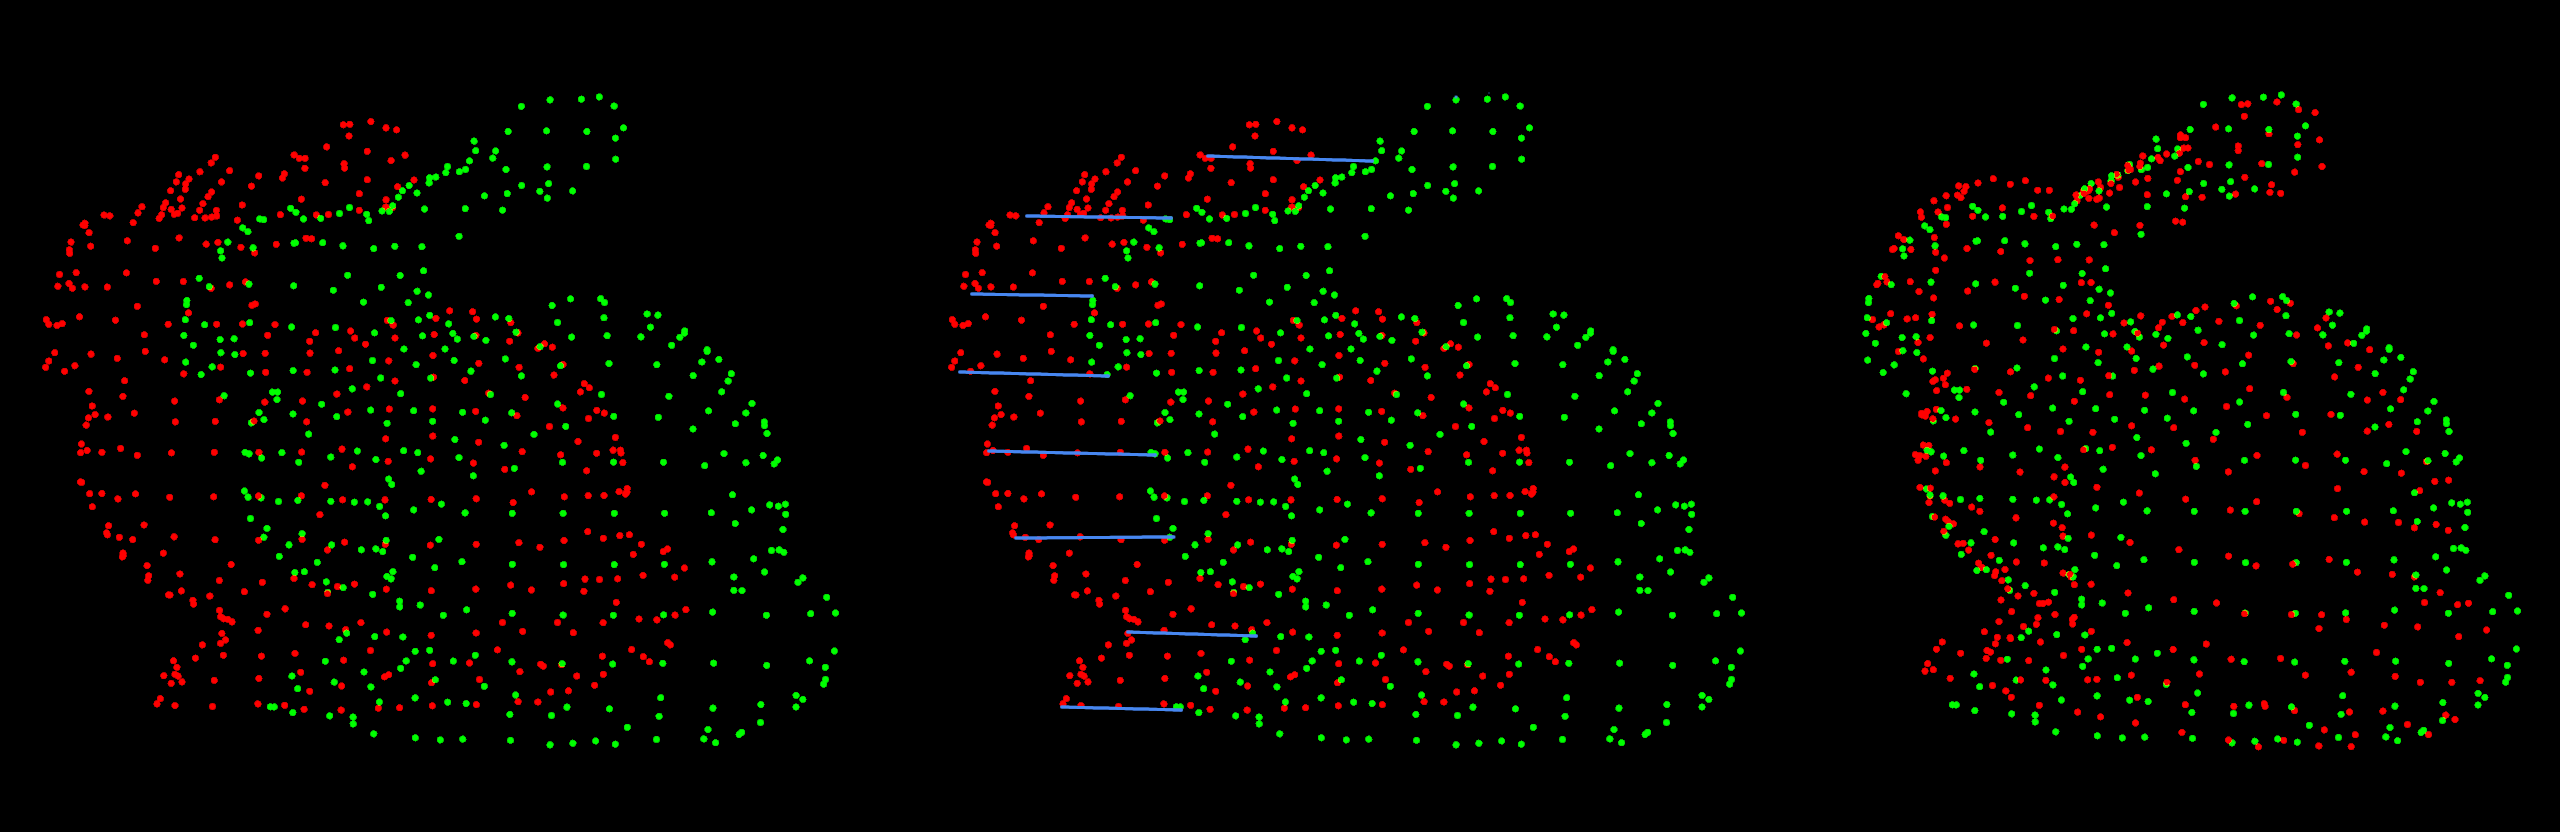
\includegraphics[scale=0.15]{registration_bunny}
\caption{Ejemplo de alineamiento de dos nubes de puntos.}\label{fig:registration_bunny}
\end{figure}
\\
\\
Para conocer en mayor detalle el proceso de alineamiento, se muestra en la figura \ref{fig:registration_flow} el conjunto de pasos que se siguen desde que se indican las nubes de entrada hasta que se obtiene la fusión de las mismas.

\begin{figure}
\centering
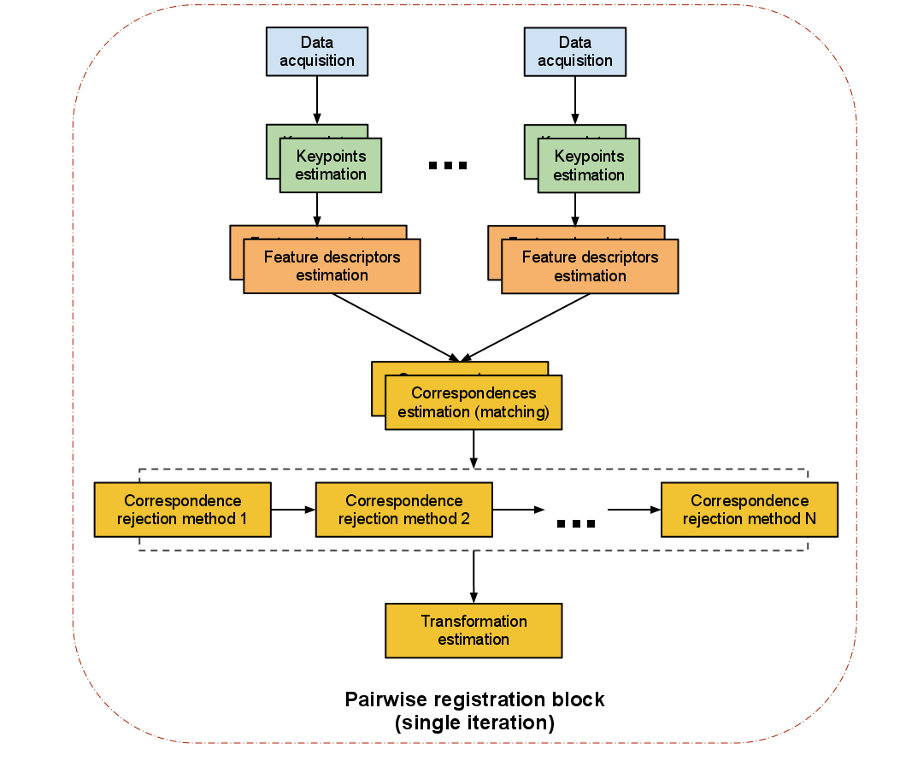
\includegraphics[scale=0.5]{registration_flow}
\caption{Procedimiento completo para llevar a cabo el alineamiento de nubes de puntos.}\label{fig:registration_flow}
\end{figure}

\subsubsection{Extracción de puntos clave}
Se explica ahora el proceso de estimación de puntos clave\cite{puntos_clave}. Una vez se han adquirido dos o más nubes de puntos como entrada, se procede a extraer keypoints o puntos clave de cada una de ellas. Por keypoint, punto clave o punto de interés se entiende como un punto de la nube que representa características especiales de la misma tal y como son esquinas o bordes. Por lo tanto, las principales características de un keypoint pueden resumirse en los siguientes puntos:
%https://en.wikipedia.org/wiki/Interest_point_detection
\begin{itemize}
\item[•] Tiene una clara definición matemática.
\item[•] Tiene una clara definición de su posición en el espacio.
\item[•] El entorno local alrededor del keypoint es rico en información característica de la nube de modo que el uso del keypoint simplifica el uso de la misma.
\item[•] Es estable ante perturbaciones locales y globales tal y como cambios de iluminación y brillo de modo que las operaciones aplicadas sobre estos puntos tengan elevada repetibilidad.
\item[•] De forma opcional, el keypoint puede incluir un atributo de escala para poder aplicar operaciones sobre keypoints obtenidos de imágenes reales así como poder tolerar cambios de escala.
\end{itemize}

%COMPLETAR CON http://www.pointclouds.org/assets/uploads/cglibs13_features.pdf
Por ejemplo, las esquinas detectadas en una nube de puntos o imagen pueden considerarse puntos clave pues muestran información característica\cite{puntos_clave_pwp} sobre las delimitaciones del objeto detectado tal y como se aprecia en la figura \ref{fig:corner_detection}. Una esquina puede definirse como un punto cuyo entorno toma dos direcciones dominantes y diferentes entre sí, es decir, una esquina es la intersección de dos bordes siendo un borde un cambio brusco del brillo en la imagen o en el caso, la nube de puntos. Por lo tanto, las esquinas son consideradas puntos de interés invariantes a la traslación, rotación y cambios de iluminación. 
Aunque las esquinas suponen una pequeña fracción de la nube, contienen la información más importante sobre la misma la cual se puede utilizar para labores de restauración de la nube o minimizar el tamaño o número de puntos.
\begin{figure}
\centering
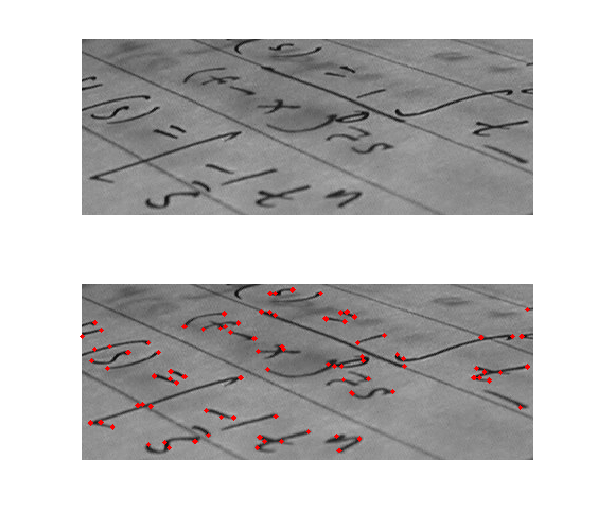
\includegraphics[scale=0.5]{corner_detection}
\caption{Ejemplo de detección de puntos clave en forma de esquinas.}\label{fig:corner_detection}
\end{figure}
\\
\\
Se ha seleccionado el proceso de obtención de keypoints mediante el algoritmo Scale Invariant Feature Transform (SIFT)\cite{sift_opencv} utilizado en visión por computador para la extracción de características (features) locales en una imagen o nube de puntos. Las aplicaciones de este algoritmo son varias como reconocimiento de objetos, navegación, modelado 3D, reconocimiento de gestos o identificación de individuos. Este algoritmo es de alta robustez y consistencia porque puede identificar objetos y características incluso en ambientes borrosos, confusos o sometidos a oclusión parcial porque se trata de un algoritmo invariante a cambios de escala, orientación, cambios de iluminación y parcialmente invariante a la distorsión afín, es decir, puede trabajar con partes de una nube de puntos cuya única diferencia es su orientación mientras que el resto de atributos permanecen idénticos.
\\
\\
Obtener correctamente los keypoints es de vital importancia ya que intentar alinear dos nubes considerando todos y cada uno de sus puntos puede suponer una carga computacional inconcebible para el caso de nubes de cientos de miles o incluso millones de puntos. 

\subsubsection{Estimación de descriptores de características}
El siguiente paso indicado en la figura \ref{fig:registration_flow} indica la estimación de los feature descriptors, es decir, los vectores donde se almacenan las características de la nube entorno a cada keypoint para poder compararlos entre sí. Por ejemplo se puede tener un vector que contiene normales a la superficie en cada keypoint o bien información sobre el brillo o luminosidad.

\subsubsection{Estimación de correspondencias}
Una vez que se dispone de dos o más vectores de características, cada uno de una nube de puntos diferente, se pasa al siguiente paso en el que hay que encontrar la información equivalente entre vectores, es decir, las características de las nubes que pueden solaparse ya que son muy parecidas o idénticas. Dependiendo del tipo de característica que se quiera alinear o unificar existen diferentes métodos para encontrar correspondencias\cite{paper_registration}
\begin{itemize}
\item[•]Emparejamiento por fuerza bruta.
\item[•]Búsqueda del vecino más cercano mediante la librería FLANN.
\item[•]Método de correspondencia directa (por defecto) Busca correspondencias en la nube modelo para todos y cada uno de los puntos de la nube fuente.
\item[•]Método de correspondencia recíproca con el que se buscan similitudes a la nube modelo en la nube fuente y viceversa quedándose solamente con la intersección.
\end{itemize}

No todas las correspondencias establecidas son correctas o de utilidad y es por esto por lo que hay que hacer una criba en el siguiente paso ya que las correspondencias inadecuadas pueden afectar negativamente a la transformación final. Para ello simplemente se puede utilizar una fracción del número total de correspondencias o utilizar algunos criterios de rechazo como los siguientes\cite{paper_registration}:
\begin{itemize}
\item[•]Rechazo basado en la \textbf{distancia}:
Se filtran correspondencias de la nube fuente si están a una distancia mayor que un valor determinado de su punto equivalente en la nube objetivo.
\item[•]Rechazo basado en \textbf{compatibilidad de normales}:
Utilizando la información sobre las normales en cada punto, se rechazan correspondencias con vectores normales inconsistentes, es decir, si el ángulo entre la normal en el punto de la nube fuente y la normal en su punto equivalente en la nube objetivo supera cierto valor.
\item[•]Rechazo basado en \textbf{correspondencias múltiples}: 
Varios puntos de la nube de entrada se corresponden con un único punto de la nube modelo. Para paliar esta situación, se suele escoger el punto de la nube de entrada más cercano al punto correspondiente en el modelo.
\item[•]Rechazo basado en \textbf{solapamiento}:
La nube fuente y la nube objetivo tienen un solapamiento parcial, aparecen correspondencias en puntos límite o frontera de dicho solapamiento dando lugar a errores posteriores. Una vez detectadas, estas correspondencias son eliminadas. 
\end{itemize}

Estos criterios de criba de correspondencias pueden apreciarse visualmente en la figura \ref{fig:metodos_criba}
\begin{figure}
\centering
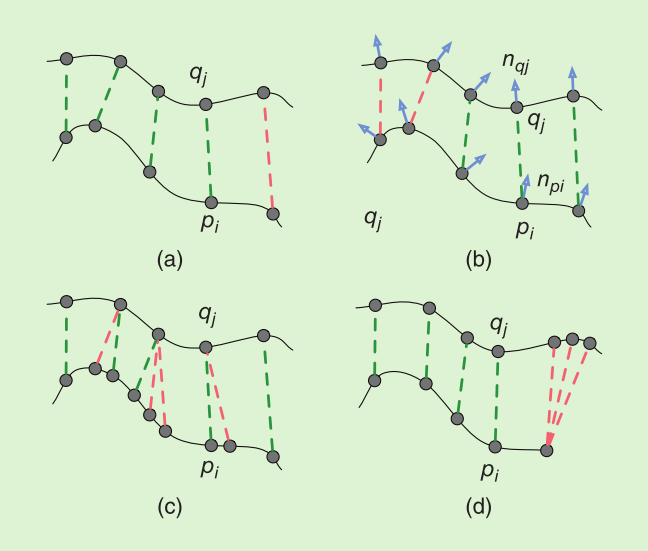
\includegraphics[scale=0.5]{metodos_criba}
\caption{Ejemplo de criba de correspondencias. Los puntos de la nube objetivo se representan como $q_j$ y los de la nube fuente como $p_i$. Se representan las técnicas de rechazo basado en la distancia (a), compatibilidad de normales (b), correspondencias múltiples (c) y solapamiento (d)}\label{fig:metodos_criba}
\end{figure}

\subsubsection{Estimación de la transformación}
En el último paso, se lleva a cabo la transformación de la nube fuente siguiendo estos puntos\cite{paper_registration}:
\begin{itemize}
\item[•]Evaluar el error existente entre los puntos de la nube fuente y sus equivalentes en la nube modelo (por ejemplo, la distancia que los separa cuando ambas nubes se representan en el mismo espacio)
\item[•]Estimar una transformación rígida de la nube fuente (es decir, conservando distancias y ángulos dentro de la misma nube) para minimizar el error evaluado anteriormente.
\item[•]Realizar la transformación de forma iterativa hasta converger a una solución aceptable.
\item[•]Optimizar la estructura de puntos resultante eliminando información redundante, por ejemplo.
\end{itemize}

Existen tres principales tipos de errores\cite{paper_registration} entre un punto de la nube fuente y su equivalente en la nube objetivo y que pueden visualizarse en la figura \ref{fig:tipos_errores} 
\begin{itemize}
\item[•]Error de distancia punto a punto:
Se trata de la distancia geométrica entre el punto de la nube fuente y su equivalente en la nube objetivo.

$$E_{punto\_punto}(T)=\sum_{k=1}^{N} w_{k}\| Tp_{k}-q_{k} \|^2$$

Donde $T$ es la matriz de transformación, $(p_{k},q_{k})$ es la $k-ésima$ de las $N$ correspondencias entre los puntos $p_k$ de la nube fuente y los puntos $q_k$ de la nube modelo. De forma opcional, se puede añadir un factor de peso $w_k$ para dar más o menos importancia a la correspondencia de puntos.

\item[•]Error de distancia punto a plano:
Es la distancia entre el punto de la nube fuente y el plano descrito por su punto equivalente junto a su vector normal en la nube objetivo.

$$E_{punto\_plano}(T)=\sum_{k=1}^{N} w_{k} ((Tp_{k}-q_{k})n_{qk}) ^2$$

Donde $T$ es la matriz de transformación, y $n_{qk}$ es el vector normal al plano.

\item[•]Error generalizado:
Es una generalización de los dos tipos de errores anteriores. Utiliza las matrices de covarianzas de los entornos locales del punto de la nube fuente y su equivalente de la nube objetivo para alinear superficies en vez de puntos.

$$E_{generalizado}(T)=\sum_{k=1}^{N} {{d_{k}}^{(T)}}^{T} (\Sigma_{k}^{Q}+T\Sigma_{k}^{P}T^{T})^{-1}d_{k}^{(T)}$$

Donde $d_{k}^{(T)}=q_{k}-Tp_{k}$ son las distancias entre las correspondencias de los puntos $(p_{k},q_{k})$, $T$ es la matriz de transformación y $T^T$ es su traspuesta. Además, se hace uso de las matrices de covarianzas de todos los puntos en la nube fuente $P$ y objetivo $Q$ que son respectivamente $\Sigma_{k}^{P}$ y $\Sigma_{k}^{Q}$.
\end{itemize}
\begin{figure}
\centering
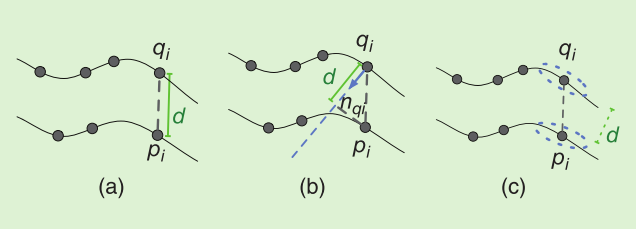
\includegraphics[scale=0.5]{tipos_errores}
\caption{Tipos de errores entre punto fuente y punto objetivo. Error de distancia punto a punto (a), error de distnacia punto a plano (b) y error generalizado (c)}\label{fig:tipos_errores}
\end{figure}

Se han mencionado los términos ``iterativa'' y ``converger'' y es que la transformación de la nube fuente hasta llegar a parecerse la máximo posible a la nube modelo no es única, se lleva a cabo un proceso iterativo\cite{paper_registration}. 
\\
\\
Sean dos nubes de puntos $n-dimensionales$:
$$M=\left\lbrace m_{i} | m_{i} \in R^n,\;\;i=1,2,...,N_{m} \right\rbrace$$
$$F=\left\lbrace f_{j} | f_{j} \in R^n,\;\;i=1,2,...,N_{f} \right\rbrace$$
\\
\\
Dicha transformación puede definirse de la siguiente manera:
$$E(R,\Delta T)=\sum_{i=1}^{N_m} \sum_{j=1}^{N_f} w_{ij} \| m_{i}-(Rf_{j}+\Delta t)  \|^2$$
\\
\\
con $w_{ij}$ como el peso que determina la dureza de la transformación pues permite que haya transformación si $w_{ij}=1$ o la anula en el caso $w_{ij}=0$
\\
\\
Esta operación se repite una y otra vez hasta que se converge a una solución y para lo cual hay que establecer criterios como los siguientes:

\begin{itemize}
\item[•]Máximo número de iteraciones:
Se ajusta un valor de máximo número de iteraciones dependiendo de la complejidad de la nube. Si se supera dicho valor, significa que la operación de alineamiento diverge.
\item[•]Límite absoluto de transformación: 
La iteraciones se detienen cuando se alcanza un valor de transformación lo suficientemente diferente a la transformación inicial
\item[•]Límite relativo de transformación:
Indica la máxima diferencia entre una operación de transformación y la anterior. Si se supera dicho límite se detiene el proceso de transformación.
\item[•]Límite de iteraciones similares: 
Se establece un límite de iteraciones para las cuales la transformación realizada es muy similar, es decir, las operaciones de trasformación a penas efectúan cambios en la nube.
\item[•]Error de mínimos cuadrados relativo:
Este criterio es similar al de límite relativo de transformación pero utilizando el valor del error de mínimos cuadrados en vez de el de transformación.
\item[•]Error de mínimos cuadrados absoluto:
Este criterio es similar al de límite absoluto de transformación pero utilizando el valor del error de mínimos cuadrados en vez de el de transformación.
\end{itemize}

Se pueden visualizar estos criterios de convergencia en la figura \ref{fig:metodos_convergencia}

\begin{figure}
\centering
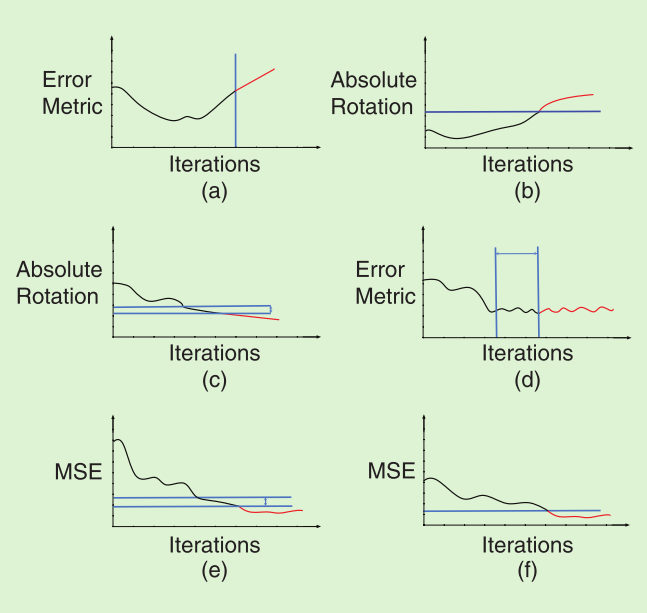
\includegraphics[scale=0.5]{metodos_convergencia}
\caption{Criterios de convergencia para la transformación iterativa. Máximo número de iteraciones (a), límite absoluto de tranformación (b), límite relativo de tranformación (c), límite de iteraciones similares (d), error de mínimos cuadrados relativo (e) y error de mínimos cuadrados absoluto (f). MSE significa Minimum Square Error, es decir, error de mínimos cuadrados.}\label{fig:metodos_convergencia}
\end{figure}

%registration with the point cloud library ---> pdf
%https://en.wikipedia.org/wiki/Harris_Corner_Detector
%https://en.wikipedia.org/wiki/Scale-invariant_feature_transform



\section{Objetivos del TFG}
Una vez establecido el fundamento teórico relativo a las nubes de puntos en general y a la librería PCL se procede a continuación a exponer el motivo de este trabajo fin de grado.
\\
\\
\textbf{El objetivo principal del trabajo es la selección y reproducción sobre un sistema embebido de un algoritmo de PCL para la extracción de puntos clave debido a la importancia del alineamiento de nubes de puntos explicada en el apartado \ref{registration}.} 
\\
\\
Un sistema embebido puede definirse como un sistema de computación diseñado para realizar una tarea o tipo de tarea en concreto, es decir, necesidades específicas, todo lo contrario a lo que es un ordenador de propósito general (ordenador personal por ejemplo) que está diseñado para cumplir un amplio rango de necesidades muy diferentes entre sí y con diferentes requerimientos de recursos.
\\
A efectos prácticos, un sistema embebido se suele construir con una placa base sobre la que se colocan todos sus recursos hardware (procesador, comunicaciones, almacenamiento etc.) mientras que un ordenador de propósito general dispone de una placa base con una serie de componentes básicos pero además dispone de otros elementos como una tarjeta gráfica, fuente de alimentación o memoria en forma modular, es decir, intercambiables y mucho más potentes.
\\
\\
Por lo tanto, cabe esperar de un sistema embebido una lista de recursos muy limitados para el procesamiento software pero con la posibilidad de acelerarlos mediante el hardware del que dispone ya que puede configurarse para realizar tareas específicas.
\\
\\
Para conseguir el objetivo mencionado, el autor divide su trabajo en las siguientes partes:
\begin{itemize}
\item[1)] \textbf{Estudio de la librería PCL:} Portar la biblioteca PCL a un sistema embebido localizando el algoritmo de extracción de puntos clave. A continuación se estudia dicho algoritmo para comprender su funcionamiento e implementación en C++ identificando dentro del mismo las operaciones necesarias para extraer keypoints. Una vez estudiadas estas operaciones, se miden sus tiempos de ejecución sobre diferentes nubes de puntos para estimar la carga computacional que suponen y así seleccionar la más pesada para acelerarla mediante hardware en el sistema embebido.

\item[2)] \textbf{Aceleración hardware:} El autor hacer uso de software para síntesis de alto nivel para describir en hardware la parte del algoritmo de extracción de keypoints que debe ser acelerada y así poder generar el archivo de configuración correspondiente para el sistema embebido.
\end{itemize}

Se tienen a continuación algunas notas importantes sobre el desarrollo del trabajo:
\begin{itemize}
\item[•] Para llevar a cabo el paso 2) previamente mencionado se utilizarán conocimientos de High Level Synthesis (HLS) que se traduce como síntesis de alto nivel y puede definirse como un proceso automatizado que interpreta una descripción algorítmica de un deseado comportamiento implementado en un lenguaje de programación de alto nivel (C o C++ por ejemplo) y crea hardware digital que implementa dicho comportamiento. De esta manera se podrá crear una Intellectual Property (IP) que contiene la optimización mencionada y así hacer uso de ella.
\item[•] La plataforma sobre la que se comprobará la compleción de dichos objetivos es un sistema en chip: chip que integra un conjunto de elementos prefabricados con funcionalidades diferentes y que pueden verse como cajas negras que tienen señales de entrada y salida. Entre los elementos que pueden incluirse en un sistema en chip destacan el microprocesador, bloque FPGA, memoria, reloj o interfaces de comunicación.
\item[•] Como objetivo adicional, haciendo uso de la librería PCL se reproduce sobre un ordenador de propósito general el algoritmo correspondiente de PCL para visualizar nubes de puntos por pantalla así como sus keypoints. Este objetivo se lleva a cabo para poder apreciar visualmente los resultados de la extracción de puntos clave y no se desarrolla sobre el sistema embebido puesto que no dispone de interfaz gráfica debido a sus recursos limitados.
\end{itemize}

\section{Organización de la memoria}
La memoria del trabajo consta de un total de seis capítulos teniendo en cada uno de estos el siguiente contenido y exceptuando lo ya visto en el presente capítulo:
\\
\\
\textbf{Capítulo 2, Herramientas empleadas para la realización del proyecto:} Se trata de la definición y explicaciones necesarias sobre las herramientas utilizadas durante el desarrollo del trabajo y por qué se han elegido.
\\
\\
\textbf{Capítulo 3, Implementación de un pipeline de visulaización y procesamiento de nubes de puntos:} En este capítulo se explica en primer lugar como es el proceso de compilación de bibliotecas de PCL para proceder a la explicación sobre cómo,haciendo uso de esta biblioteca, se han implementado dos programas que sirven para visualizar nubes de puntos y extraer keypoints de las mismas.
\\
\\
\textbf{Capítulo 4, Medición de tiempos de ejecución de algoritmos de PCL:} Se explica de forma genérica cómo se pueden medir tiempos de ejecución de algoritmos haciendo uso de las librerías adecuadas  y se aplica dicho método a los algoritmos involucrados en el proceso de extracción de keypoints. Esto sirve para determinar cuál es el de mayor carga computacional, esto es, el que más tiempo lleva su ejecución para ser implementado en hardware digital y así poder ser acelerado.
\\
\\
\textbf{Capítulo 5, Análisis del algoritmo de extracción de normales usando PCL:} Se explica el algoritmo seleccionado en el capítulo anterior tanto a nivel teórico como práctico (cómo se lleva a cabo en la librería PCL) Una vez comprendido el funcionamiento del mencionado algoritmo, se selecciona una de sus partes para ser acelerada mediante hardware digital atendiendo a los criterios de la síntesis de alto nivel y la aceleración de operaciones triviales y de elevada frecuencia como puede ser cualquier tipo de operación aritmética.
\\
\\
\textbf{Capítulo 6, Implementantación de la extracción de normales mediante síntesis de alto nivel:} En este capítulo se plantea el fragmento original (de la librería PCL) del algoritmo seleccionado para su aceleración para contrastar los cambios que el autor efectúa sobre el mismo para que se posible su sínteis en hardware digital. A continuación, se explica cómo se genera la IP de aceleración de hardware utilizando Vivado así como se muestra la validación de su correcto funcionamiento sobre la placa de desarrollo Pynq-Z1.


\section{Conclusiones}
Se ha visto en este capítulo el fundamento teórico referente a las nubes de puntos, el software existente para procesar tal información y algunas de sus capacidades.
\\
Además, se han expuesto los objetivos del presente trabajo y en el siguiente capítulo se explicarán las principales herramientas necesarias para conseguirlos.






